\chapter{Theoretical Calculations}
\label{chap:Theory_Predictions}

In an experiment, the measurements are validated by doing the comparison with the perturbative QCD (pQCD) theoretical calculations. The lowest order (LO) calculations describe well the shapes of the measured distributions but not the normalization due to the dependence on the unphysical renormalization (\mur) and factorization (\muf) scales. The next-to-leading order calculations (NLO) improves the precision by reducing the dependence on \mur and \muf scales and become an essential feature in the determination of fundamental parameters such as $\alpha_S$ and the parton distribution functions (PDF). This chapter describes the next-to-leading order pQCD calculations used for comparison with the measurements. NLO pQCD calculations need to be corrected for the multiparton interactions (MPI) and hadronization effects by applying non-perturbative (NP) corrections and also for the electroweak interactions (EW).

\section{Fixed Order NLO Calculations}
The predictions of the inclusive differential jet event cross-section at NLO accuracy in pQCD are computed with the \NLOJETPP program version~4.1.3~\cite{Nagy:2001fj,Nagy:2003tz}. The results are provided within the framework of \fastNLO version~2.3~\cite{Kluge:2006xs,Britzger:2012bs}. The PDFs are accessed through the \LHAPDFS library \cite{Whalley:2005nh,Buckley:2014ana}. The \fastNLO is preferred over the direct calculation with \NLOJETPP because with \fastNLO the calculations of the cross-sections can be repeated several times with different PDFs and scale choices required for calculating the PDF and scale uncertainties. Here the factorization and renormalization scales are chosen equal to \httwo, i.e. \muf = \mur = \httwo. 

In the current study, different PDF sets available for a series of different assumptions on the strong coupling constant at the scale of the $Z$ boson mass \alpsmz are used for NLO calculations. Table~\ref{tab:nlopdfsets} summarizes the already existing PDF sets in LHC Run~1 (upper rows) and the newer PDF sets for Run~2 (lower rows). The different columns list the number of flavours $N_f$, the assumed masses $M_t$ and $M_Z$ of the top quark and the $Z$ boson, respectively, the default values of \alpsmz, and the range in \alpsmz variation available for fits for different PDF sets. All sets uses a variable-flavour number scheme with at most five or six flavours apart from the ABM11 PDFs, which employ a fixed-flavour number scheme with $\NF=5$. Out of these eight PDF sets the following three are not considered further because of the below mentioned reasons :

\begin{itemize}
\item At NLO, predictions based on ABM11 do not describe LHC jet data at small jet rapidity \cite{Aad:2013lpa, Aad:2014vwa, CMS:2014mna, Khachatryan:2015luy}.
\item The HERAPDF2.0 set exclusively fits HERA DIS data with only weak constraints on the gluon PDF.
\item The range in values available for \alpsmz is too limited for the NNPDF3.0 set.
\end{itemize}

Mainly CT10 PDF set is considered for comparison between data and theory predictions as well as for calculating theoretical uncertainties. 

\begin{table}[htbp]
 \centering
 \caption{NLO PDF sets are available via \LHAPDFS with various assumptions on the value of \alpsmz. The upper rows list the already existing sets in LHC Run~1 and newer ones for Run~2 are listed in lower rows, along with the corresponding number of flavours $N_f$, the assumed masses $M_t$ and $M_Z$ of the top quark and the $Z$ boson, respectively, the default values of \alpsmz, and the range in \alpsmz variation available for fits.}
 \label{tab:nlopdfsets}
 \vspace{2mm}
 \begin{tabular}{lccllc}
 \hline\hline
 Base set & \NF & $M_t$ (\GeVns{}) & $M_Z$ (\GeVns{}) &\alpsmz & \alpsmz range\rbthm\\  \hline
 % LHC Run 1
 ABM11 \cite{Alekhin:2012ig}                 &  5        & 180       & 91.174  & $0.1180$   & 0.110 - 0.130\rbtrr\\
 CT10  \cite{Lai:2010vv}                     & ${\leq}5$ & 172       & 91.188  & $0.1180$ & 0.112 - 0.127\rbtrr\\
 MSTW2008 \cite{Martin:2009iq,Martin:2009bu} & ${\leq}5$ & $10^{10}$ & 91.1876 & $0.1202$   & 0.110 - 0.130\rbtrr\\
 NNPDF2.3 \cite{Ball:2012cx}                 & ${\leq}6$ & 175       & 91.1876 & $0.1180$ & 0.114--0.124\rbtrr\\\hline
 % LHC Run 2
 CT14 \cite{Dulat:2015mca}                   & ${\leq}5$ & 172       & 91.1876 & $0.1180$ & 0.111--0.123\rbtrr\\
 HERAPDF2.0 \cite{Abramowicz:2015mha}        & ${\leq}5$ & 173       & 91.1876 & $0.1180$ & 0.110--0.130\rbtrr\\
 MMHT2014 \cite{Harland-Lang:2014zoa}        & ${\leq}5$ & $10^{10}$ & 91.1876 & $0.1200$ & 0.108--0.128\rbtrr\\
 NNPDF3.0 \cite{Ball:2014uwa}                & ${\leq}5$ & 173       & 91.2    & $0.1180$ & 0.115--0.121\rbtrr\\
 \hline\hline
 \end{tabular}
\end{table}

\subsection{NLO Correction Factors}
\label{sec:nlo_factors}
The differences between LO predictions and NLO predictions give the effect of the higher-order contributions to the pQCD predictions. These are described by a NLO correction factor, k\hy factor, which is derived as the ratio of cross-sections at NLO accuracy to that at LO i.e.

\begin{equation}
\label{eq:kfactors}
 {\rm k\hy factor} = \frac{\sigma_{\rm NLO}}{\sigma_{\rm LO}}
\end{equation}
%i.e. ${\rm k\hy factor}_{\ratio} = {\rm \frac{k\hy factor_{3\hy jet}}{k\hy factor_{2\hy jet}}}$. 
The impact of the higher-order corrections is determined by the size of k-factor. The small size of k-factor indicates that the cross-section predictions are precisely described at the LO whereas the larger size hints the contributions from NLO. Figure~\ref{fig:kfactor} shows the k-factors of the \NLOJETPP calculations, for inclusive 2-jet and 3-jet event cross-sections and their ratio \ratio, using five different PDF sets. k-factor for \ratio is obtained by taking the ratio of k-factors for inclusive 3-jet event cross-sections to that of inclusive 2-jet. The k-factors are similar for all the PDF sets in the lower region, but the differences increase in regions with larger \httwo. It is observed that for inclusive 3-jet event cross-sections, k-factor jumps at lowest \httwo. This is because some jet configurations are kinematically forbidden near the \pt cut bin i.e. 150 GeV. Since the first few bins in \httwo (below 225 GeV) still suffer from these kinematical effects, the minimum value of \httwo studied is 300 GeV.

\begin{figure}[!htbp]
 \begin{center}
 \hspace*{-5mm}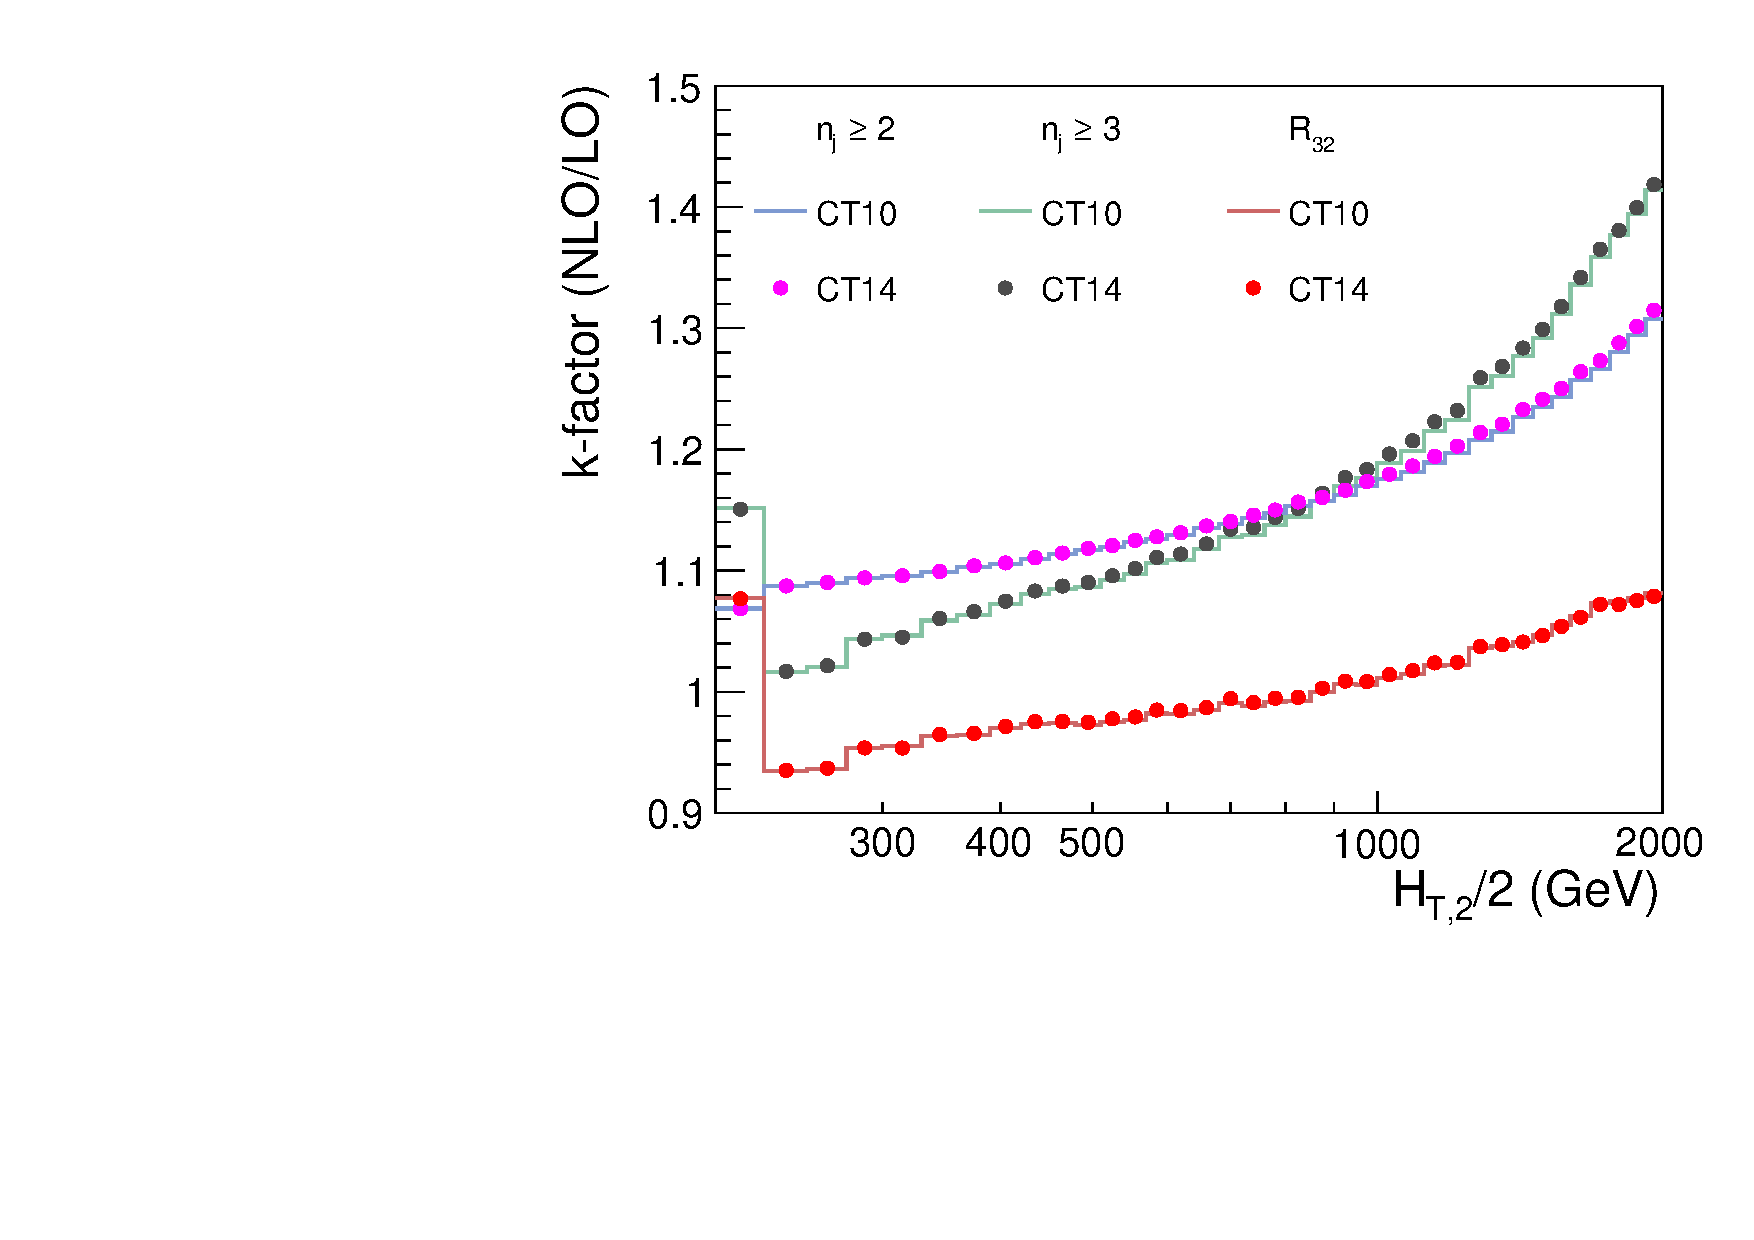
\includegraphics[width=0.51\textwidth]{Plots_HT_2_150/Kfactor_all_1.pdf}%
 ~~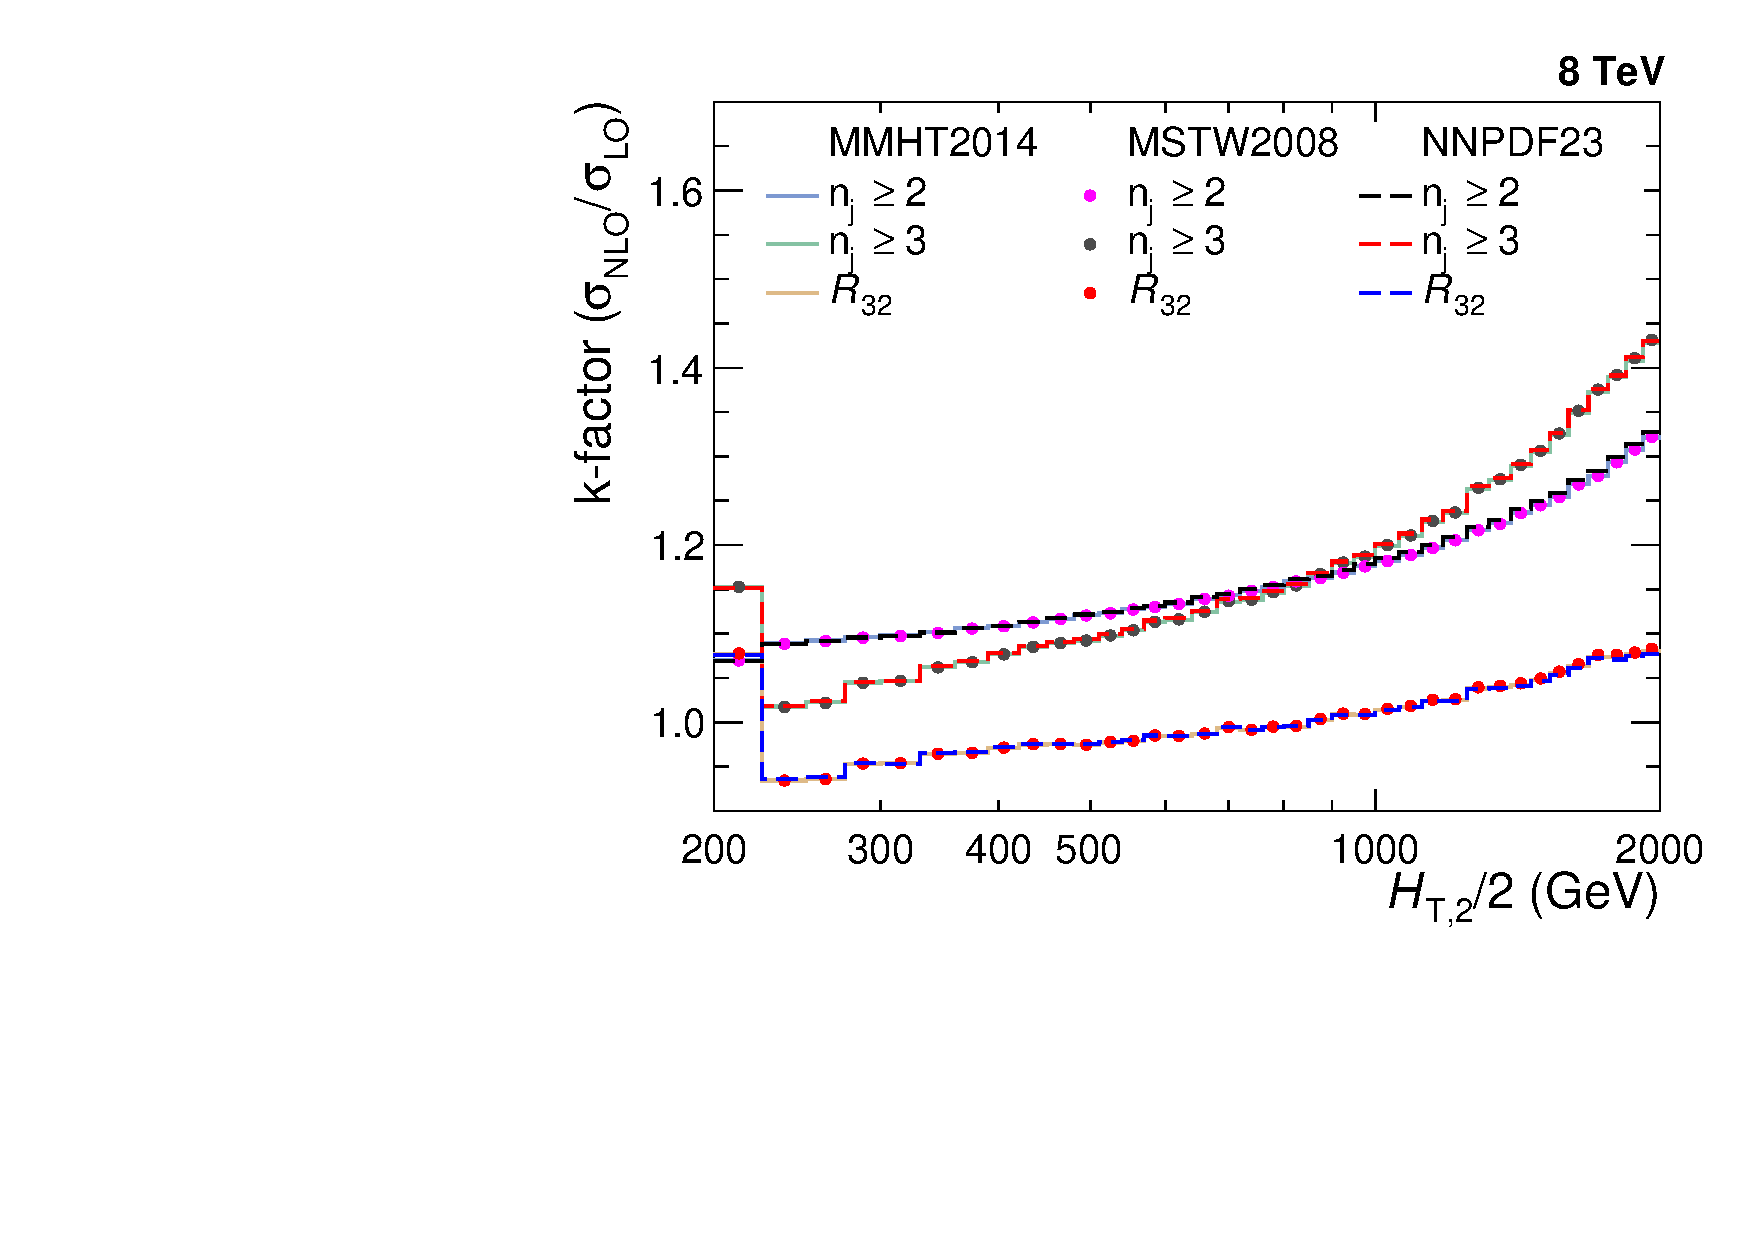
\includegraphics[width=0.51\textwidth]{Plots_HT_2_150/Kfactor_all_2.pdf}
 \caption[]{The k-factors of the \NLOJETPP calculations, for inclusive 2-jet and 3-jet event cross-sections and their ratio \ratio, using five different PDF sets.}
 \label{fig:kfactor}
 \end{center}
\end{figure}

\subsection{Non-Perturbative Corrections}
\label{sec:NPcorr}

The fixed-order pQCD NLO calculations predict the parton-level cross-section but lacks accuracy due to several effects. The partons which are emitted close to each other in phase space are not handled well in lower order perturbation theories and hence requires a parton shower (PS) correction. The scattering phenomena between partons within a colliding proton, other than the hard scattering, give rise to multi-parton interactions (MPI). The partons of the hard scattering forms colorless bound states called hadrons through a process of hadronization (HAD). The MPI and hadronization cannot be modelled well within the perturbative framework. Since the fixed-order NLO calculations do not include these additional soft QCD effects, these calculations cannot be compared directly to unfolded data. So the corrections for non-perturbative effects (NP) should be taken into account in NLO calculations. The ratio of cross-section predicted with a nominal event generation interfaced to the simulation of UE contributions and to the one without hadronization and MPI effects gives the NP correction factors which are defined as : 

\begin{equation}
 \label{Eq:np}
 C^{\rm NP} = \frac{\sigma^{\rm PS \plusn HAD \plusn MPI}}{\sigma^{\rm PS}}
\end{equation}

In the current study, the NP effects are estimated by using samples obtained from various MC event generators with a simulation of parton shower and underlying-event (UE) contributions. The leading order (LO), \HERWIGPP with the default tune of version 2.3 and \PYTHIAS with tune \Ztwostar, and the NLO \POWHEG MC event generators are considered. The matrix-element calculation is performed with \POWHEG interfaced to \PYTHIAE with tune CUETS1 for the UE simulation. The ratio, defined in Eq.~\ref{Eq:np}, is obtained for each MC generator and is fitted by a power-law function defined in Eq.~\ref{Eq:power}. Since this ratio obtained from different MC generators have large differences, so the average of the envelope, which covers all the differences, is taken as the correction factor which is then applied as bin-by-bin multiplicative factor to the parton-level NLO cross-section. The half of the envelope it is taken as the uncertainty on the NP correction factor. 

\begin{equation}
 \label{Eq:power}
 f(\httwo) = a\cdot\big(\httwo\big)^{b}\plus c
\end{equation}

The NP correction factors, $C_{\rm 3\hy jet}^{\rm NP}$ and $C_{\rm 2\hy jet}^{\rm NP}$ are calculated for \njt~and \njth~event cross-sections respectively and then their ratio gives the correction factor for \ratio . The correction factors are shown in Fig.~\ref{fig:np_factors} for the inclusive 2-jet (top left) and 3-jet event cross-sections (top right), and for ratio \ratio (bottom). At \httwo $\sim$300 GeV, the NP corrections amount to $\sim$4\hy 5\% for inclusive 2-jet and 3-jet event cross-sections and $\sim$1\% for \ratio, and decrease rapidly for increasing \httwo. On comparing the NP correction factors of \ratio with that for individual cross-sections, it has been observed that the non-perturbative effects get reduced in \ratio.

\begin{figure}[!ht]
 \begin{center}
 \hspace*{-5mm}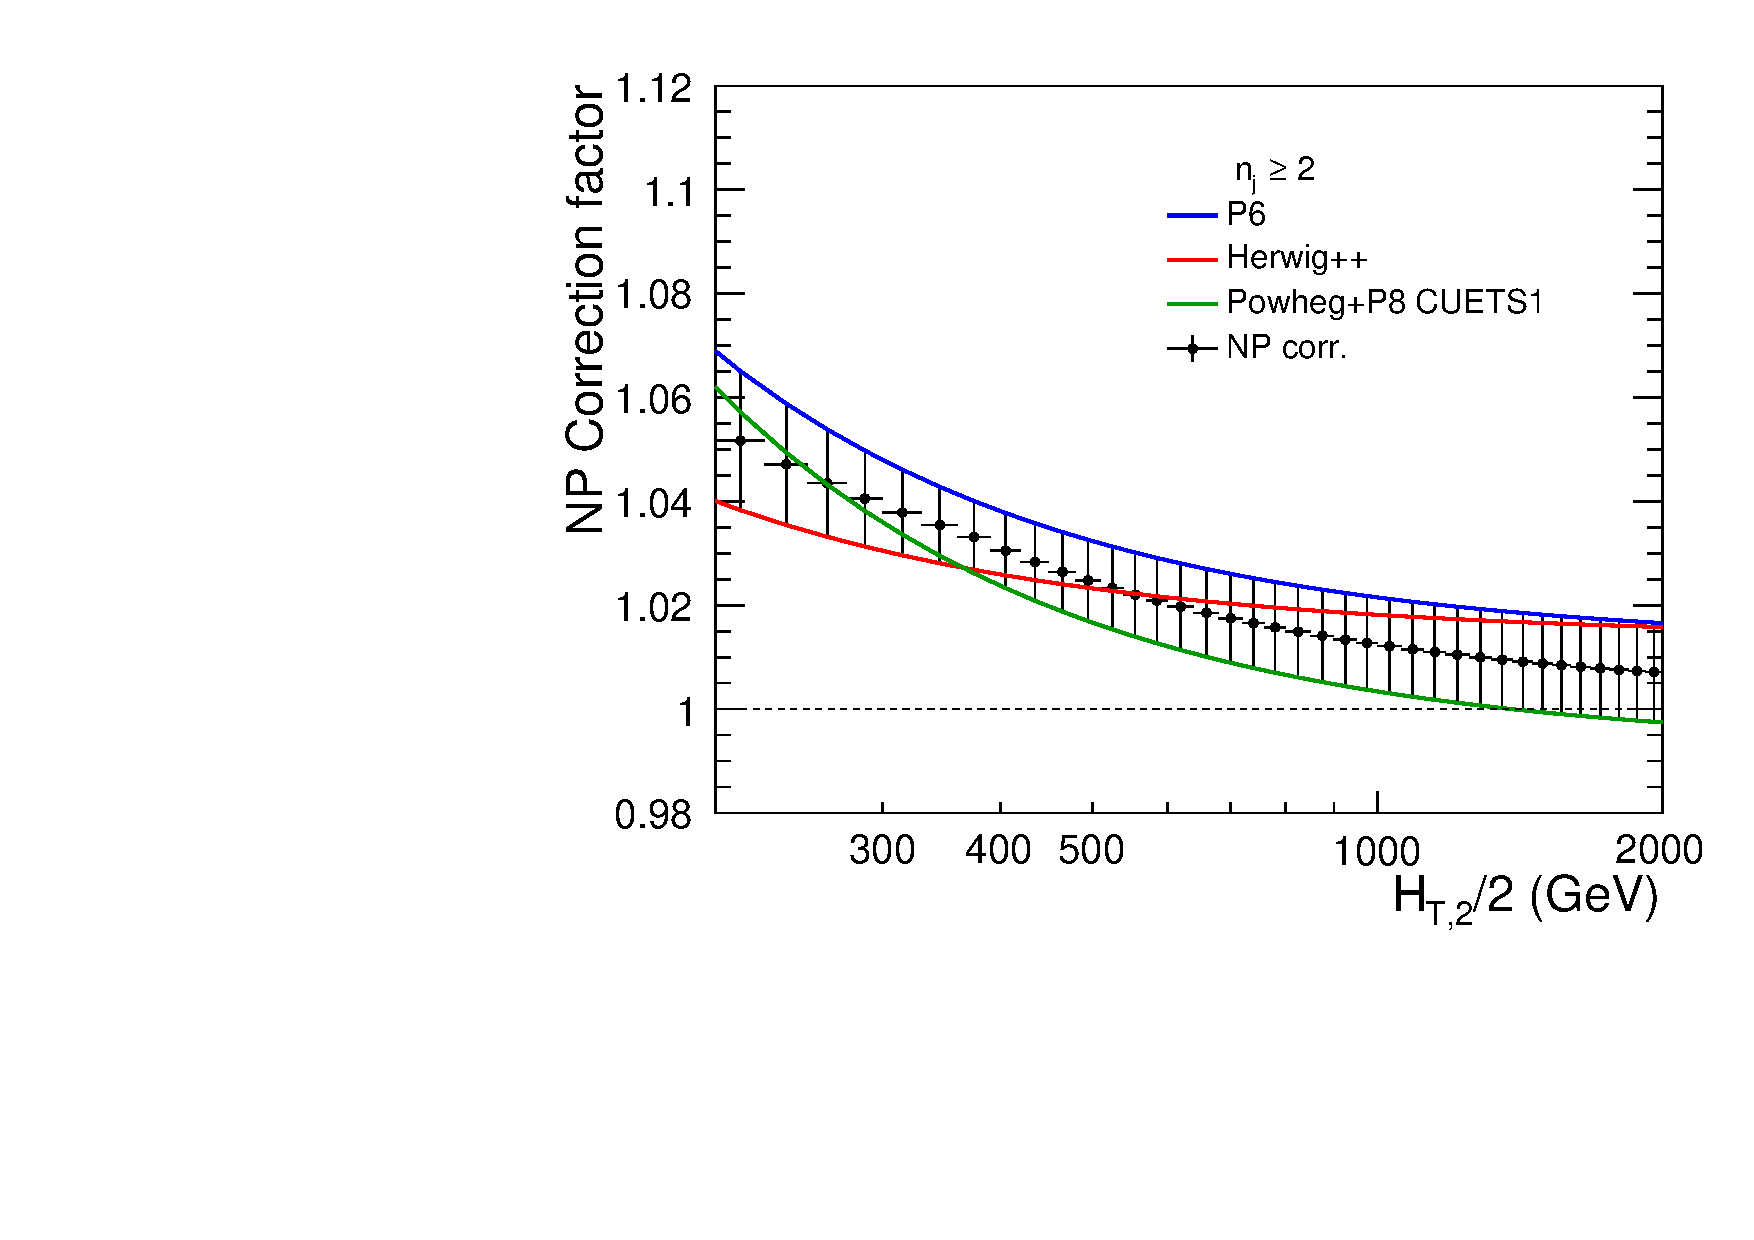
\includegraphics[width=0.51\textwidth]{Plots_HT_2_150/Final_NP_Corr_2.pdf}%
 ~~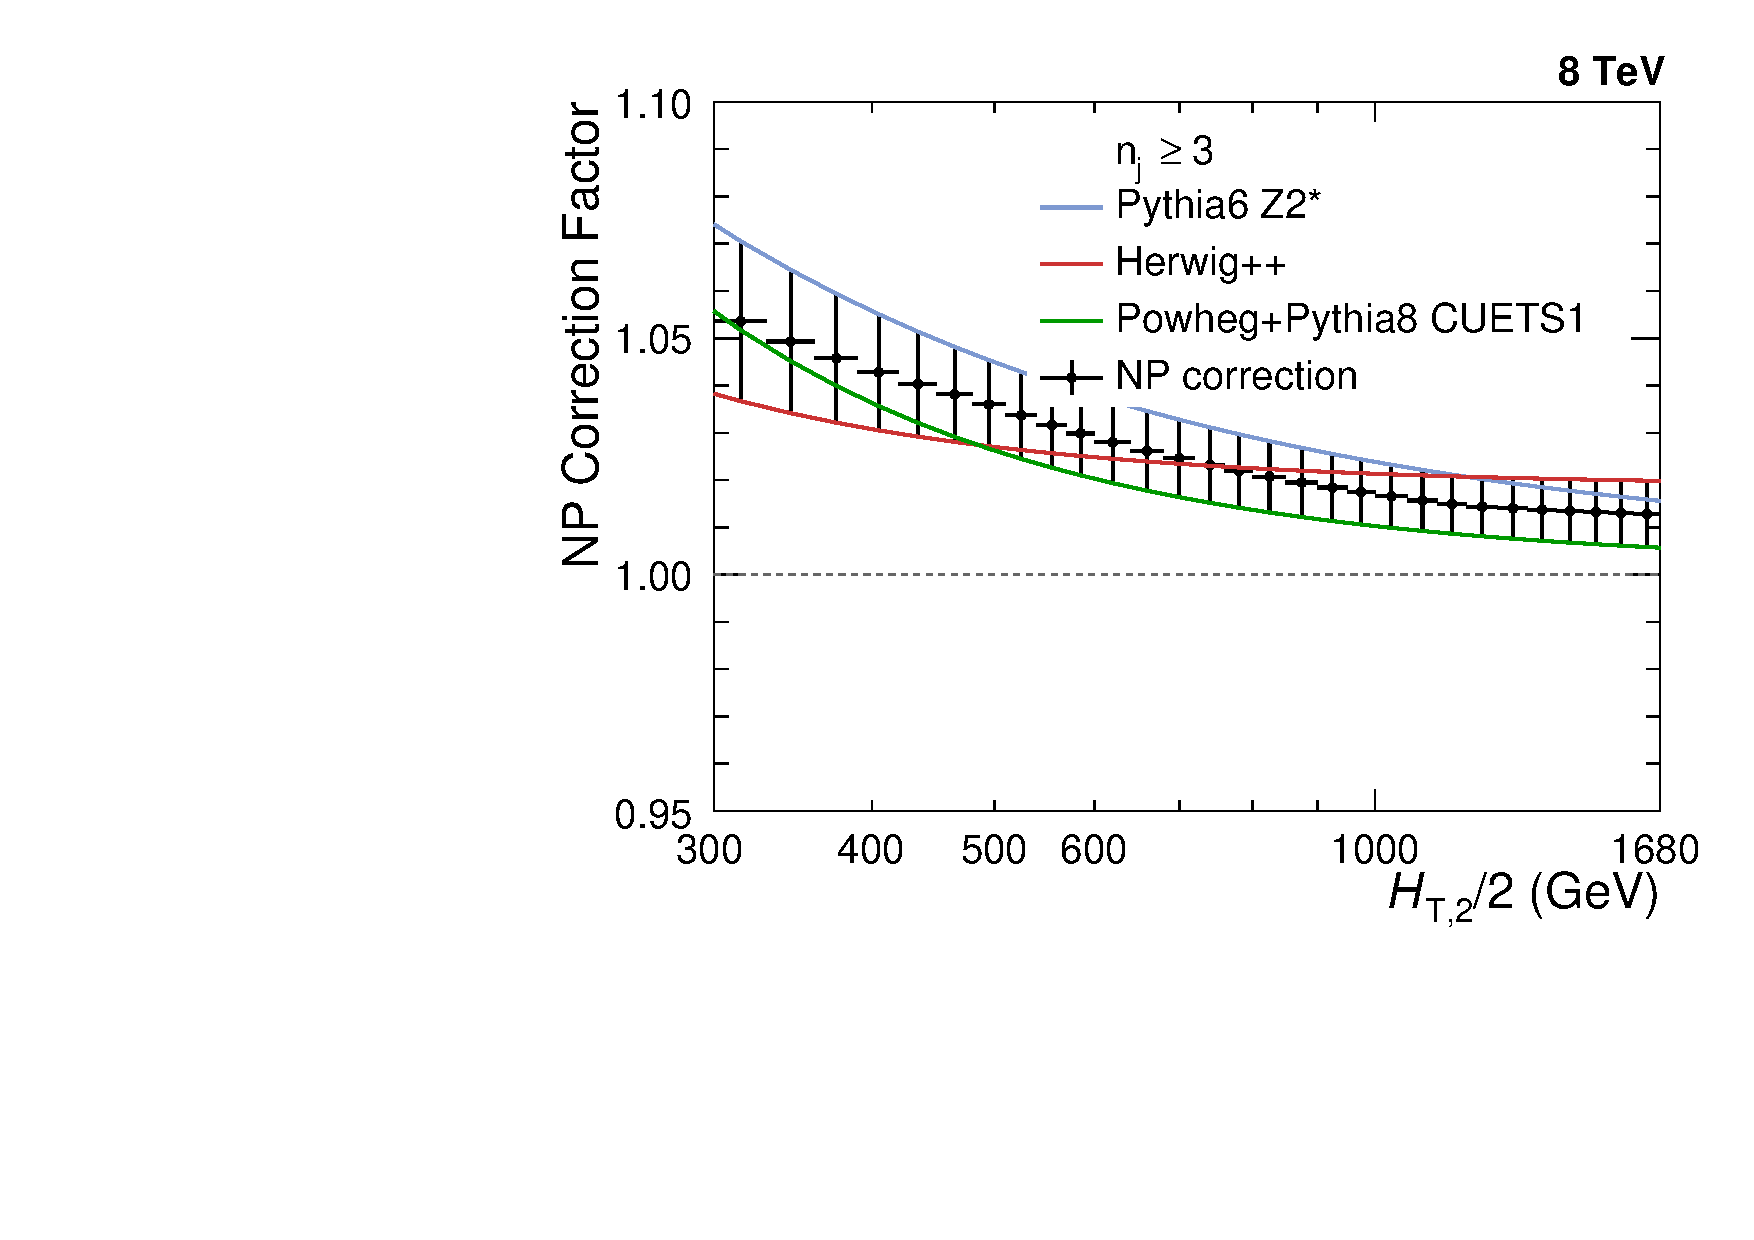
\includegraphics[width=0.51\textwidth]{Plots_HT_2_150/Final_NP_Corr_3.pdf}\\
 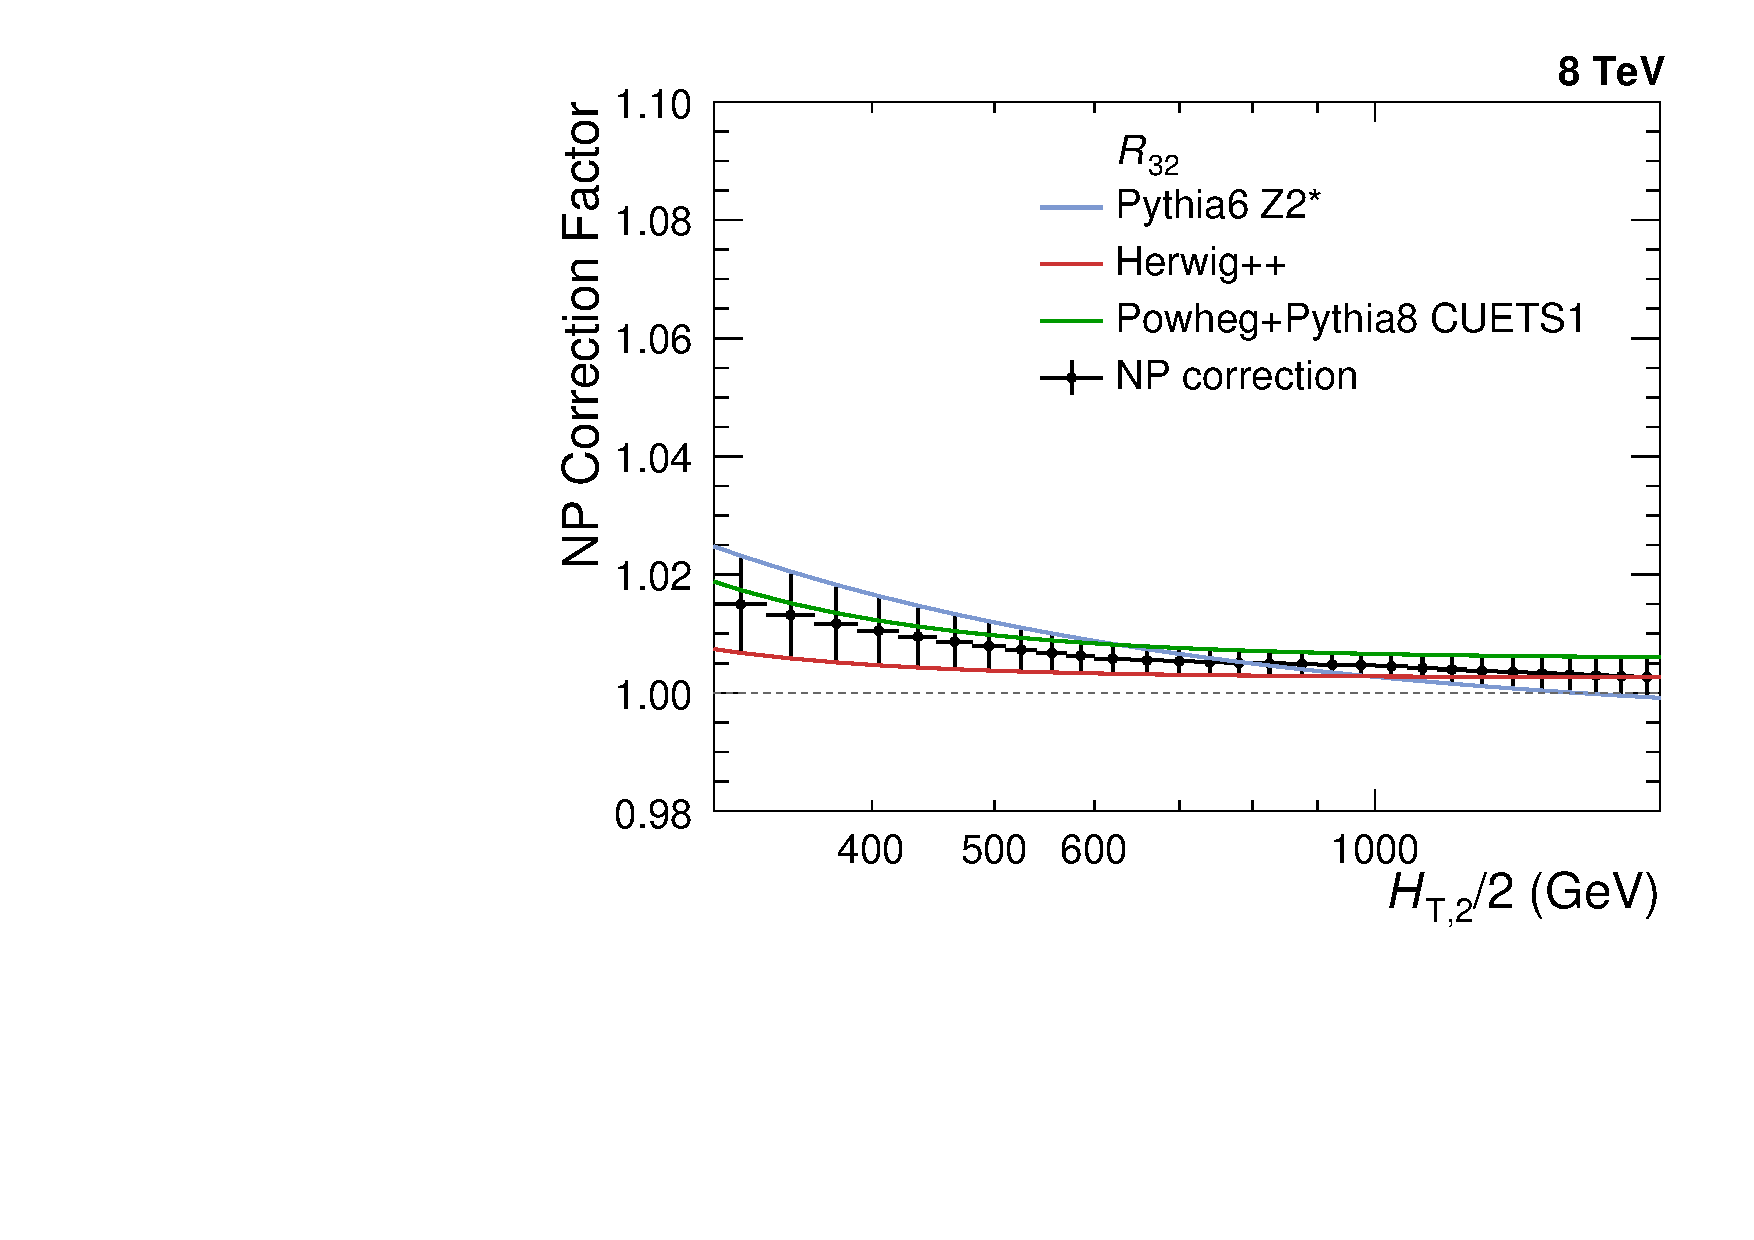
\includegraphics[width=0.51\textwidth]{Plots_HT_2_150/Final_NP_Corr_Ratio_32.pdf}
 \caption[]{The nonperturbative (NP) corrections are presented as a function of \httwo for inclusive 2-jet (top left) and 3-jet (top right) event cross-sections, as well as their ratio \ratio. These corrections are calculated from the leading order \HERWIGPP with the default tune of version 2.3 (red line) and \PYTHIAS with tune \Ztwostar (blue line); and the next-to-leading order \POWHEG interfaced to \PYTHIAE with tune CUETS1 (green line) Monte Carlo event generators. The black solid circles give the average NP correction factor along with the uncertainty shown by the error bars. }
 \label{fig:np_factors}
 \end{center}
\end{figure}
%This is because the strong coupling constant, \alpsns, decreases with increasing energy faster than the EW one as ${\rm \alpha_{W} \equiv \alpha_{EM}/sin^2 \theta_W}$ (where $\alpha_{EM}$ is the electro,agnetic (EM) coupling constant and ${\rm \theta_W}$ is the weak angle). Also the purely weak part of higher order EWeffects produces lead-ing corrections of the typeαWlog(μ2/M2W), whereinμrepresents some typical energy scaleaffecting the hard process in a given observable, e.g., the partonic CM energy√ˆ. The

\subsection{Electroweak Corrections}
\label{sec:EW}
In LHC, the centre-of-mass energy of proton-proton collisions is well beyond the electroweak (EW) scale $\sim{\cal O}$(100 GeV). At such a high energy, the impact of higher order EW corrections is much more with respect to QCD effects \cite{Hollik:2004dz} and affect jet cross-sections at large \httwo. The quark-quark scattering processes involving virtual exchanges of massive $W$ and $Z$ bosons contribute to electroweak (EW) corrections. The fixed-order QCD calculations do not include EW corrections and hence the NLO theory calculations are corrected for EW effects. The EW corrections have been calculated for inclusive 1-jet and 2-jet case, in Ref. \cite{Dittmaier:2012kx}. The EW correction factors in the phase space of the measurement are shown as a function of \httwo in Fig.~\ref{fig:EW} for inclusive 2-jet event cross-sections. These correction factor increases up to 13\% at high ends of \httwo which are applied as a bin-by-bin correction factor to the fixed-order \NLOJETPP calculations. To see the effects of EW corrections, a ratio of data to theory predictions obtained using CT10-NLO PDF set and corrected with NP effects without including EW corrections (left) and including EW corrections (right) is plotted for inclusive 2-jet event cross-sections in Fig.~\ref{fig:EW_Comp}. On comparing both the figures, it is observed that the EW corrections significantly improve the agreement between data and prediction in the high \httwo region. EW corrections are not available yet for inclusive 3-jet production and hence not applied for inclusive 3-jet event cross-sections. The guess from theory side is that EW for inclusive 2-jet and 3-jet will be similar, so for \ratio, it is assumed to be equal to the factor of 1. Since the EW effects are not taken care of in MC simulations so these corrections are applied to MC predictions also. 

\begin{figure}[!t]
 \begin{center}
 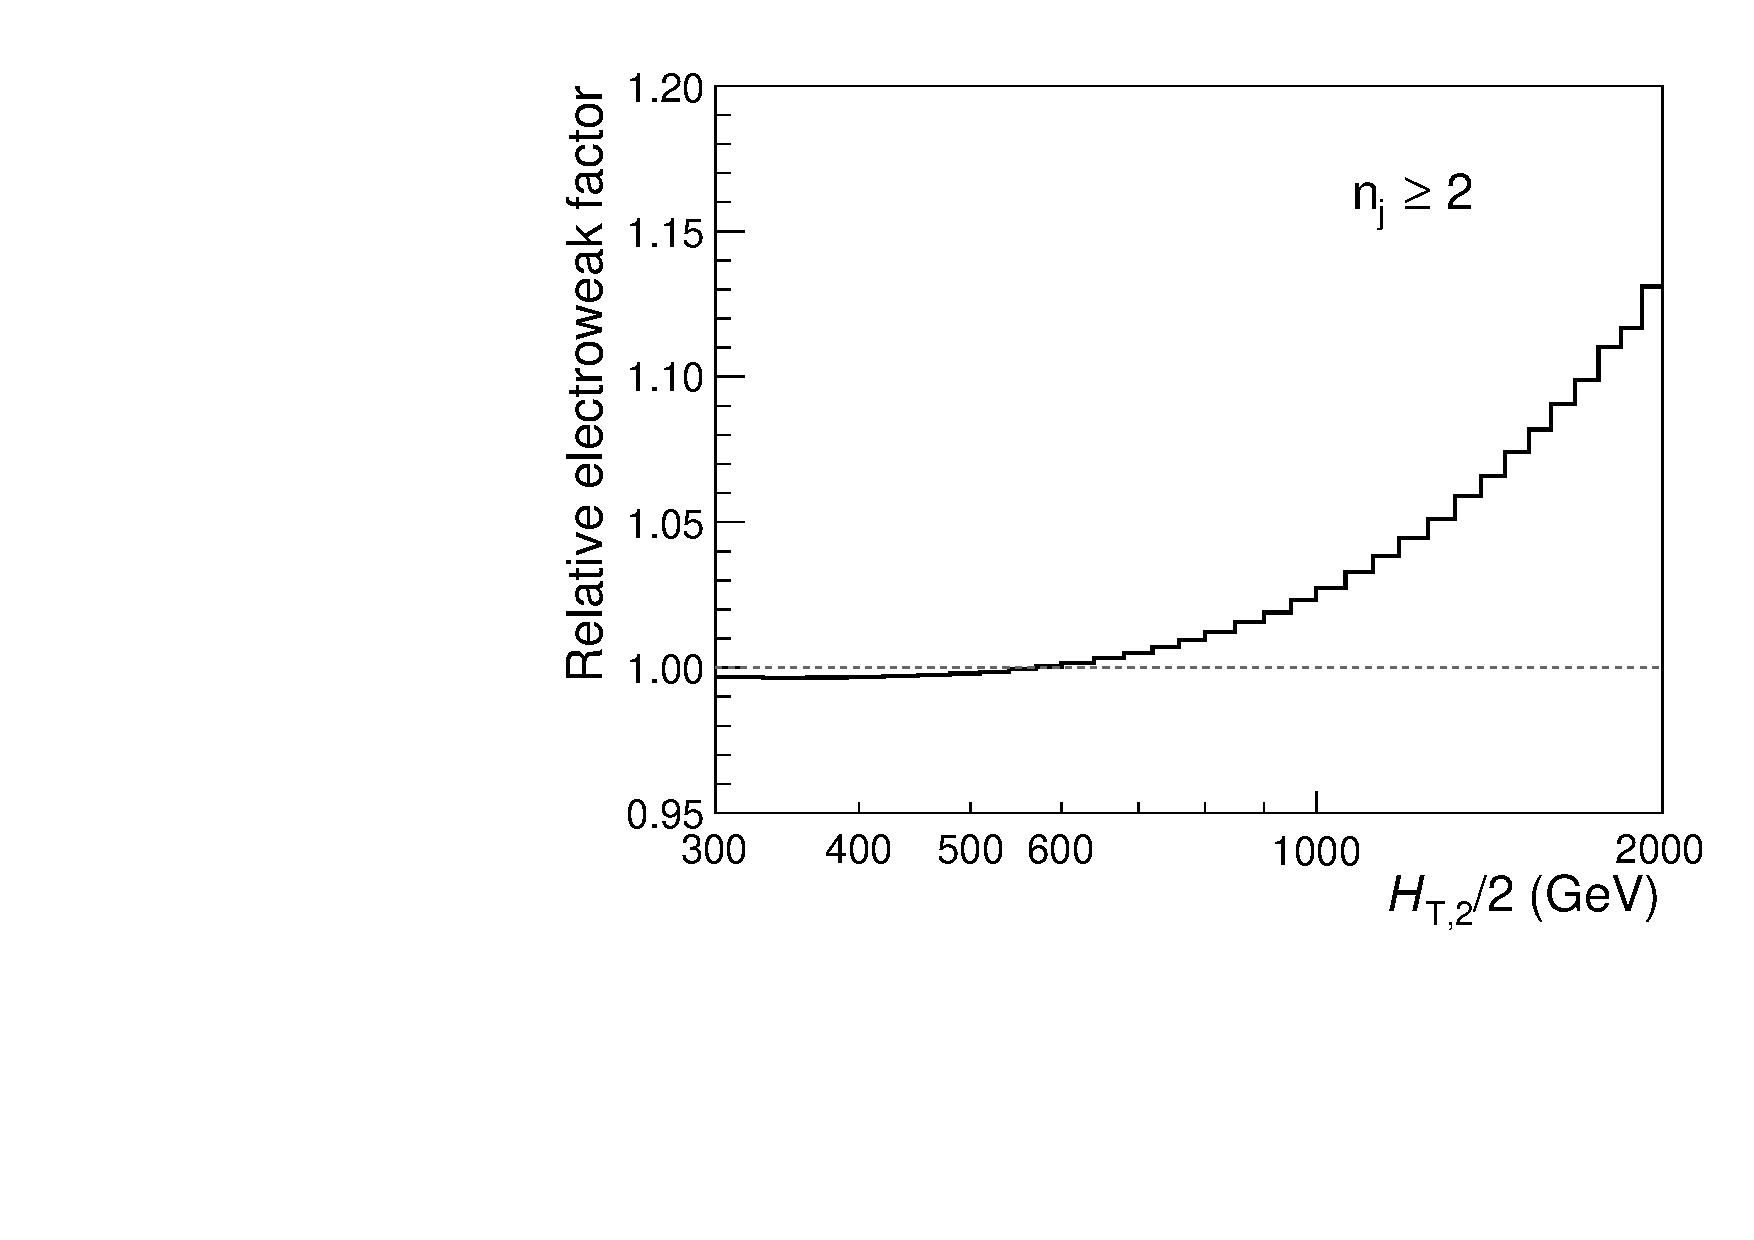
\includegraphics[width=0.51\textwidth]{Plots_HT_2_150/EW_2.pdf}
 \caption[]{The electroweak (EW) corrections \cite{Dittmaier:2012kx} in the phase space of the measurement are shown as a function of \httwo for inclusive 2-jet event cross-sections. These corrections are applied as a bin-by-bin correction factor to the fixed-order calculation of \NLOJETPP as well as the MC predictions of \MadGraphFn\plusn \PYTHIAS. The EW correction factor increases up to 13\% at high ends of \httwo and significantly improves the agreement between data and prediction.}
 \label{fig:EW}
 \end{center}
\end{figure}

\begin{figure}[!h]
 \begin{center}
 \hspace*{-5mm}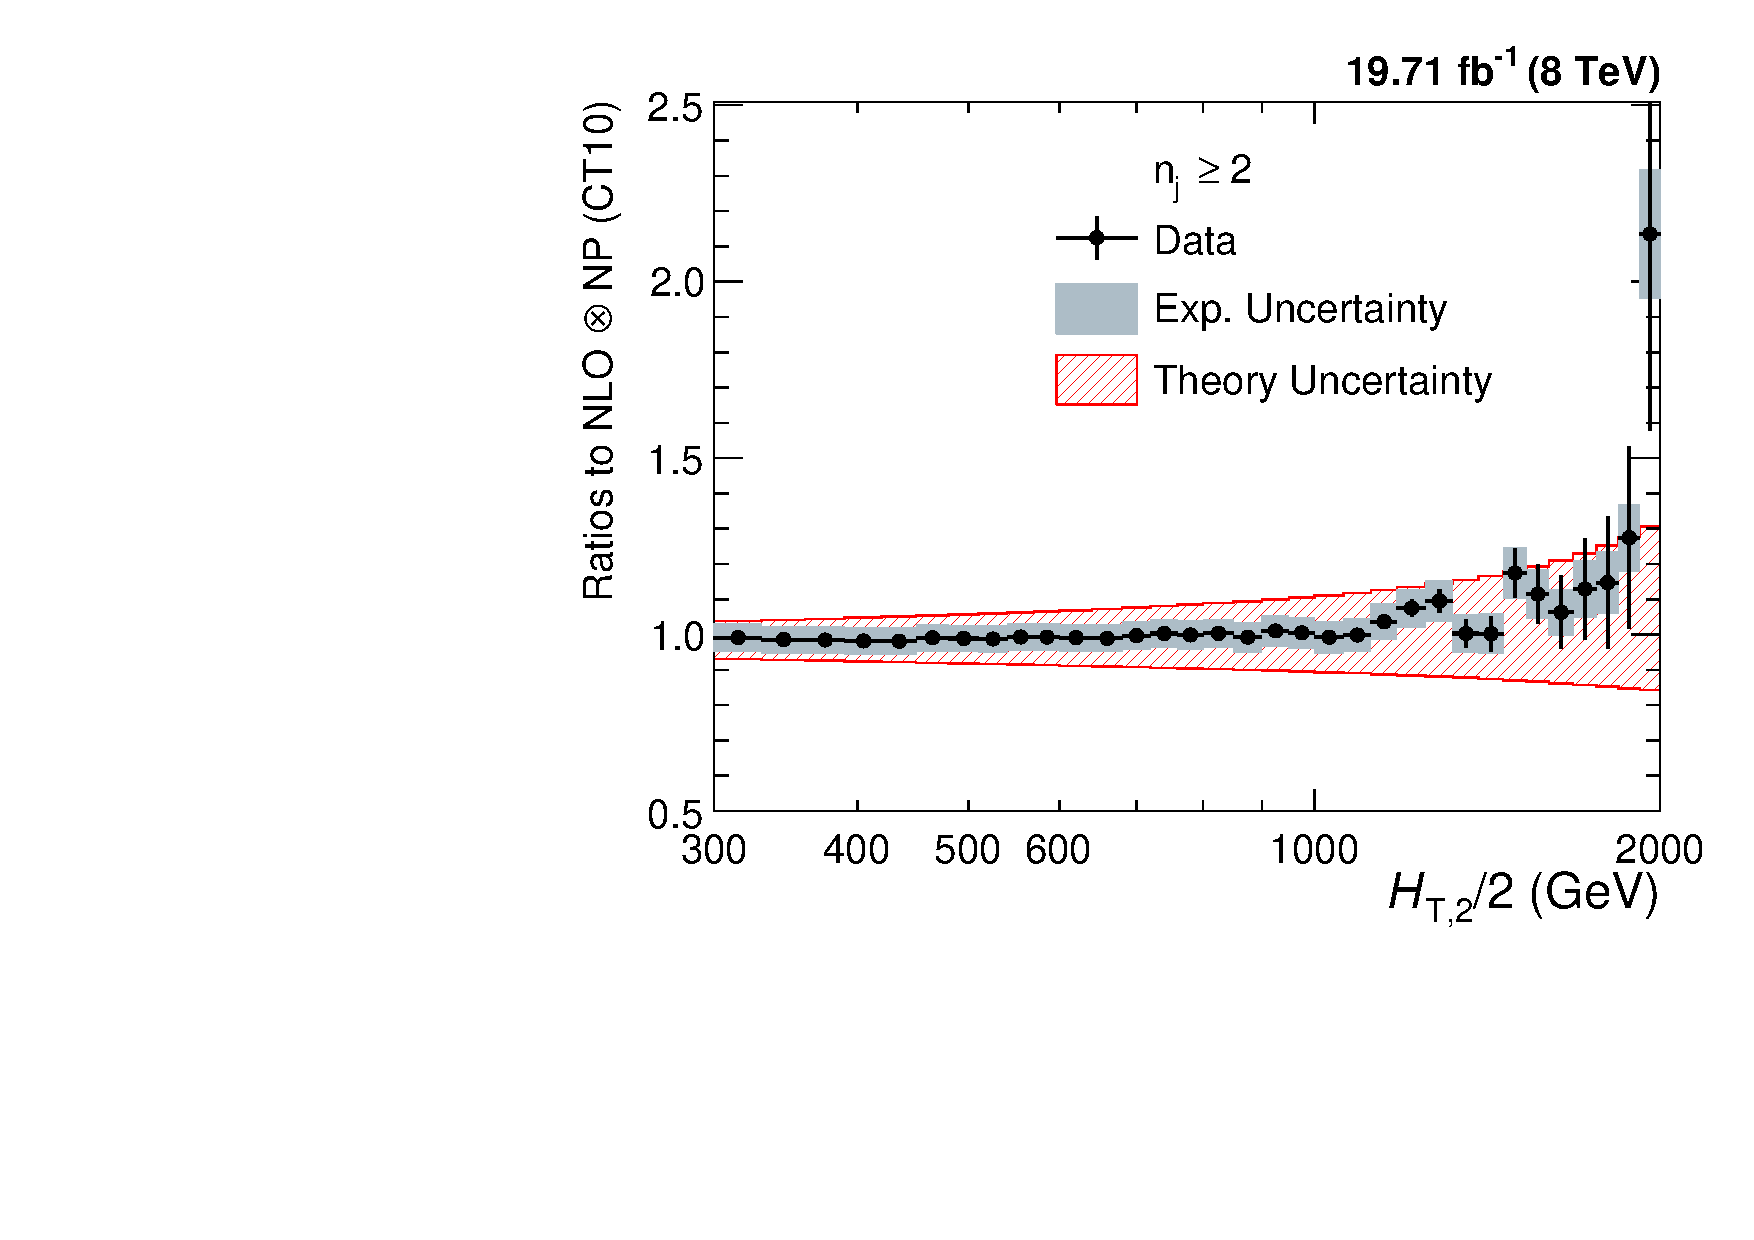
\includegraphics[width=0.5\textwidth]{Plots_HT_2_150/Comparison_data_NLO_2_NoEW.pdf}
 ~~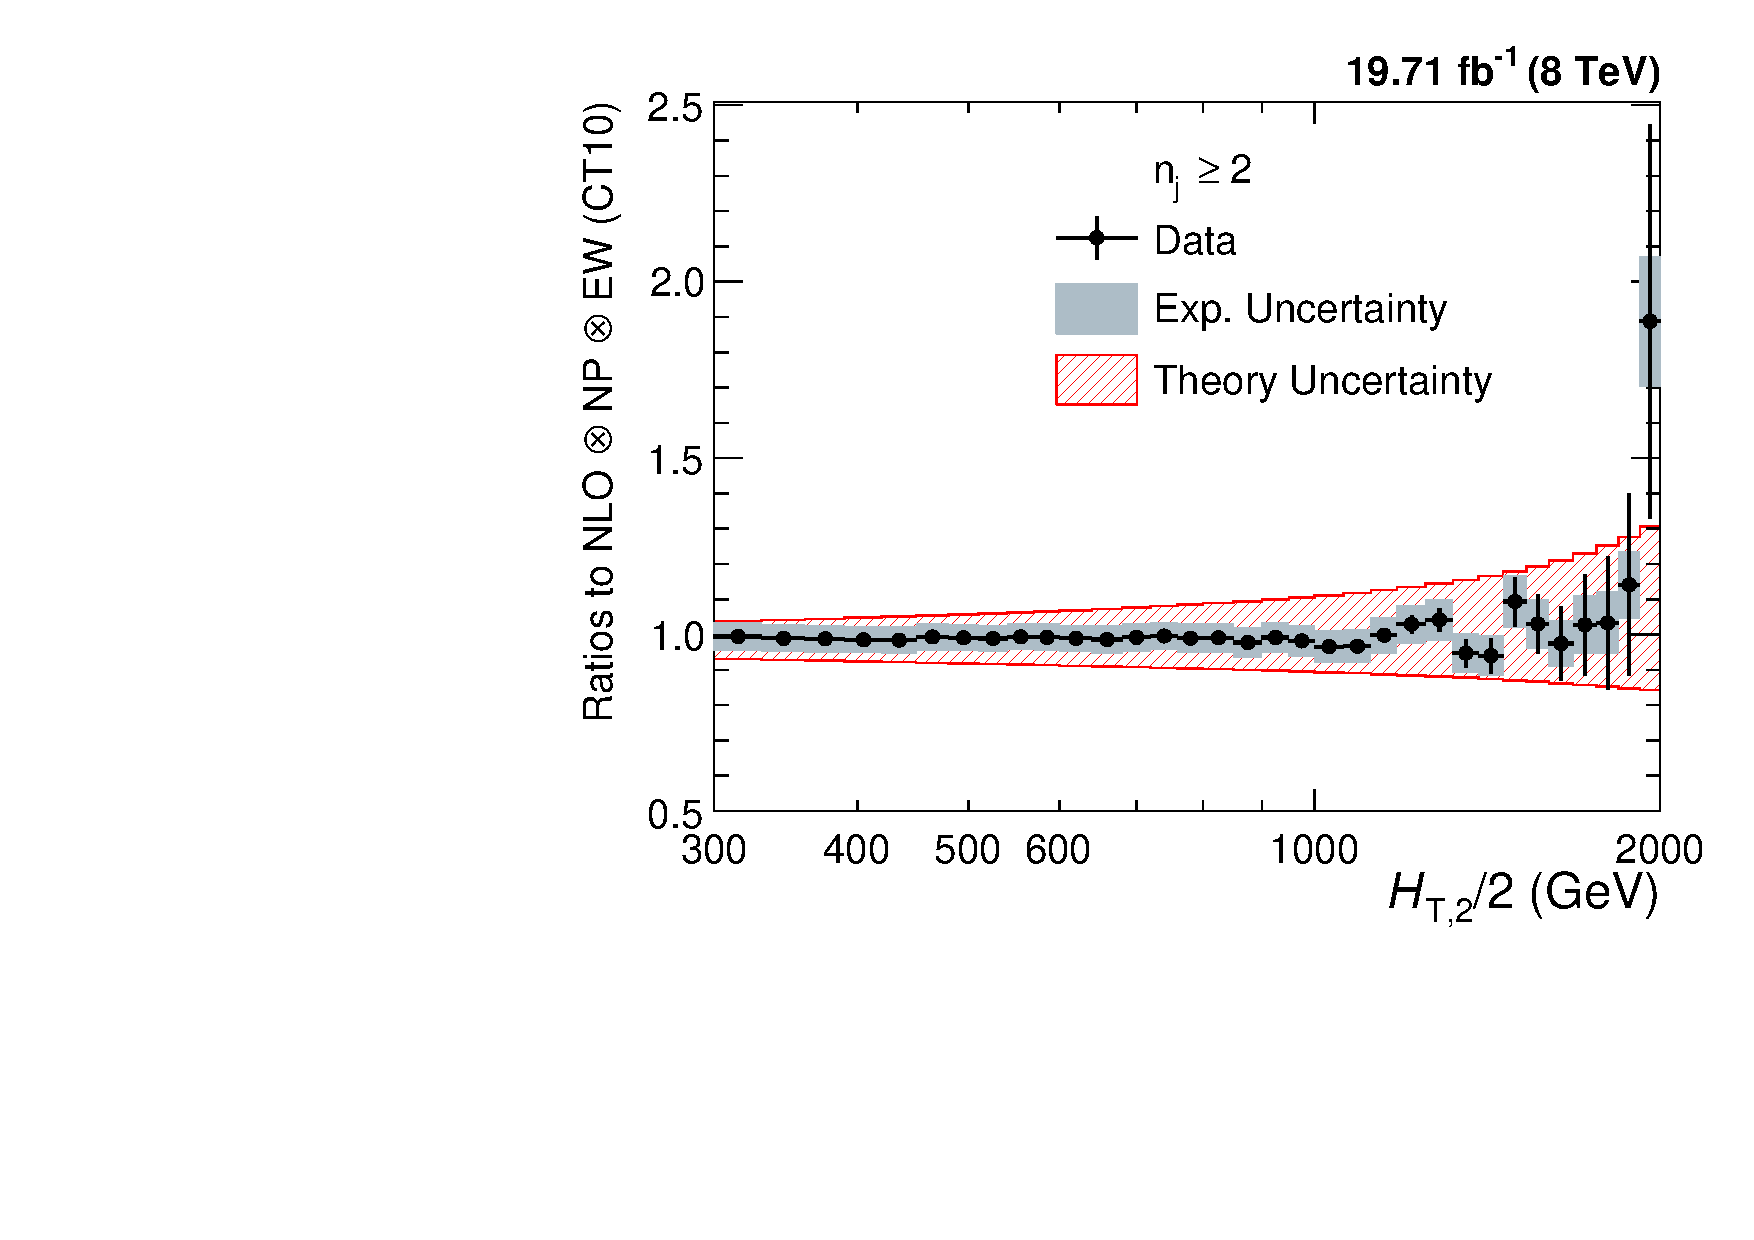
\includegraphics[width=0.5\textwidth]{Plots_HT_2_150/Comparison_data_NLO_2_EW.pdf}
 \caption[]{Ratio of data over theory obtained using the CT10-NLO PDF set and corrected with non-perturbative effects (NP) without including electroweak (EW) corrections (left) and including EW corrections (right) is shown for inclusive 2-jet event cross-sections. The error bars represents the statistical uncertainty of the data and the shaded rectangles represents the total experimental systematic uncertainty. The shaded band around unity indicate the total uncertainty of the theory. The EW corrections significantly improve the agreement between data and prediction in the high \httwo region.}
 \label{fig:EW_Comp}
 \end{center}
\end{figure}

\section{Theoretical Uncertainties}
\label{sec:theory_unc}
The measurements are not only sensitive to experimental uncertainties but also to the theoretical uncertainties. The renormalization and factorization scale variations, PDF uncertainties and the non-perturbative corrections contribute to theoretical uncertainties which are described below : 

\subsection{Scale Uncertainty}
\label{sec:scale_unc}
In perturbative QCD calculations of cross-sections, one has to choose a renormalization (\mur) and factorization (\muf) scale. The dependence on scales is negligible if these calculations are performed for all orders of the perturbative series. But the perturbative series is truncated at NLO, so there is a scale dependence of the measurement which is covered by systematic uncertainty known as scale uncertainty. The scale uncertainty is evaluated with the conventional recipe of varying the default scale \httwo chosen for \mur and \muf independently in the following six combinations: (\mur/\httwo, \muf/\httwo) = (1/2,1/2), (1/2,1), (1,1/2), (1,2), (2,1) and (2,2). The maximal upwards and downwards deviations in cross-section from the central prediction give the scale uncertainty. To calculate the scale uncertainty for cross-section ratio \ratio, first \ratio is obtained for each above mentioned scale choice and then its difference from central \ratio is taken. The scale uncertainty calculated using CT10-NLO PDF set ranges from 5\% to 13\% and 11\% to 17\% for inclusive 2-jet and 3-jet events cross-sections respectively, and from 6\% to 8\% for \ratio.

\subsection{PDF Uncertainty}
\label{sec:pdf_unc}
The calculation of jet cross-sections in proton-proton collisions relies upon the knowledge of PDFs. These PDF sets are determined by global fits to all the available deep inelastic scattering (DIS) and related hard scattering data from different experiments. The various sources affect the PDFs such as theory model, input parameters like the strong coupling constant \alpsns, the quark masses and the statistical and systematic uncertainty sources of the data included in the PDF fit. These sources contribute to PDF uncertainty which is evaluated according to the prescriptions given for each PDF set. The CT10-NLO PDF set \cite{Lai:2010vv,Pumplin:2002vw} employ the eigenvector method to evaluate the PDF uncertainties. The CT10-PDF set consists of $N_\mathrm{ev}=26$ eigenvectors with two PDF members per eigenvector $k$, which are varied upwards and downwards to generate a set of eigenvector pairs. The asymmetric uncertainties, $\Delta X^{+}$ and $\Delta X^{-}$, of a quantity X are given by Eq.~\ref{eq:unc_pdf} where $X_0$ is the central prediction, $X^{+}_k$ and $X^{-}_k$ are the predictions using the upwards and downwards variation of each eigenvector $k$. 

\begin{equation}
\label{eq:unc_pdf}
\begin{gathered}
\Delta X^+ =  \sqrt{\sum \limits_{k=1}^{N_\mathrm{ev}}\big[{\rm max}(X^{+}_{k}-X^{0},X^{-}_{k}-X^{0},0)\big]^2} \\
\Delta X^- =  \sqrt{\sum \limits_{k=1}^{N_\mathrm{ev}}\big[{\rm min}(X^{+}_{k}-X^{0},X^{-}_{k}-X^{0},0)\big]^2}
\end{gathered}
\end{equation}

The symmetric uncertainty ($\Delta X^{\pm}$) is given by half the difference of the upwards and downwards variations :

\begin{equation}
\label{eq:unc_pdf_symm}
\Delta X^{\pm} = \sqrt{\sum \limits_{k=1}^{N_\mathrm{ev}} \Bigg[\frac{X^{+}_{k}-X^{-}_{k}}{2}\Bigg]^2}
\end{equation}

The CT10-NLO PDF set uncertainties are downscaled by a factor of 1.64 in order to have the uncertainties at the 68.3\% confidence level CL(1$\sigma$) instead of 90\% CL(2$\sigma$) such that to have a uniform treatment with respect to other PDF sets. The PDF uncertainty as derived with the CT10-NLO PDF set is the dominant source of uncertainty and ranges from 3\% to 30\% for inclusive 2-jet and from 4\% to 32\% for 3-jet cross-sections. For \ratio, the ratio of predictions for inclusive 3-jet to that of 2-jet is taken for each eigen vector with upwards and downwards variations separately and then PDF uncertainty is calculated as done for individual cross-sections. The PDF uncertainty ranges and from 2\% to 10\% for cross-section ratio \ratio. 

\subsection{Non-perturbative Uncertainty}
As discussed in \ref{sec:NPcorr}, the differences in the non-perturbative (NP) corrections calculated from various Monte Carlo event generators introduce the NP uncertainty which is of the order of 1\% and 1 to 2\% for inclusive 2-jet and 3-jet event cross-sections respectively, and \ls 1\% for cross-section ratio \ratio.

\begin{figure}[!h]
 \begin{center}
 \hspace*{-5mm}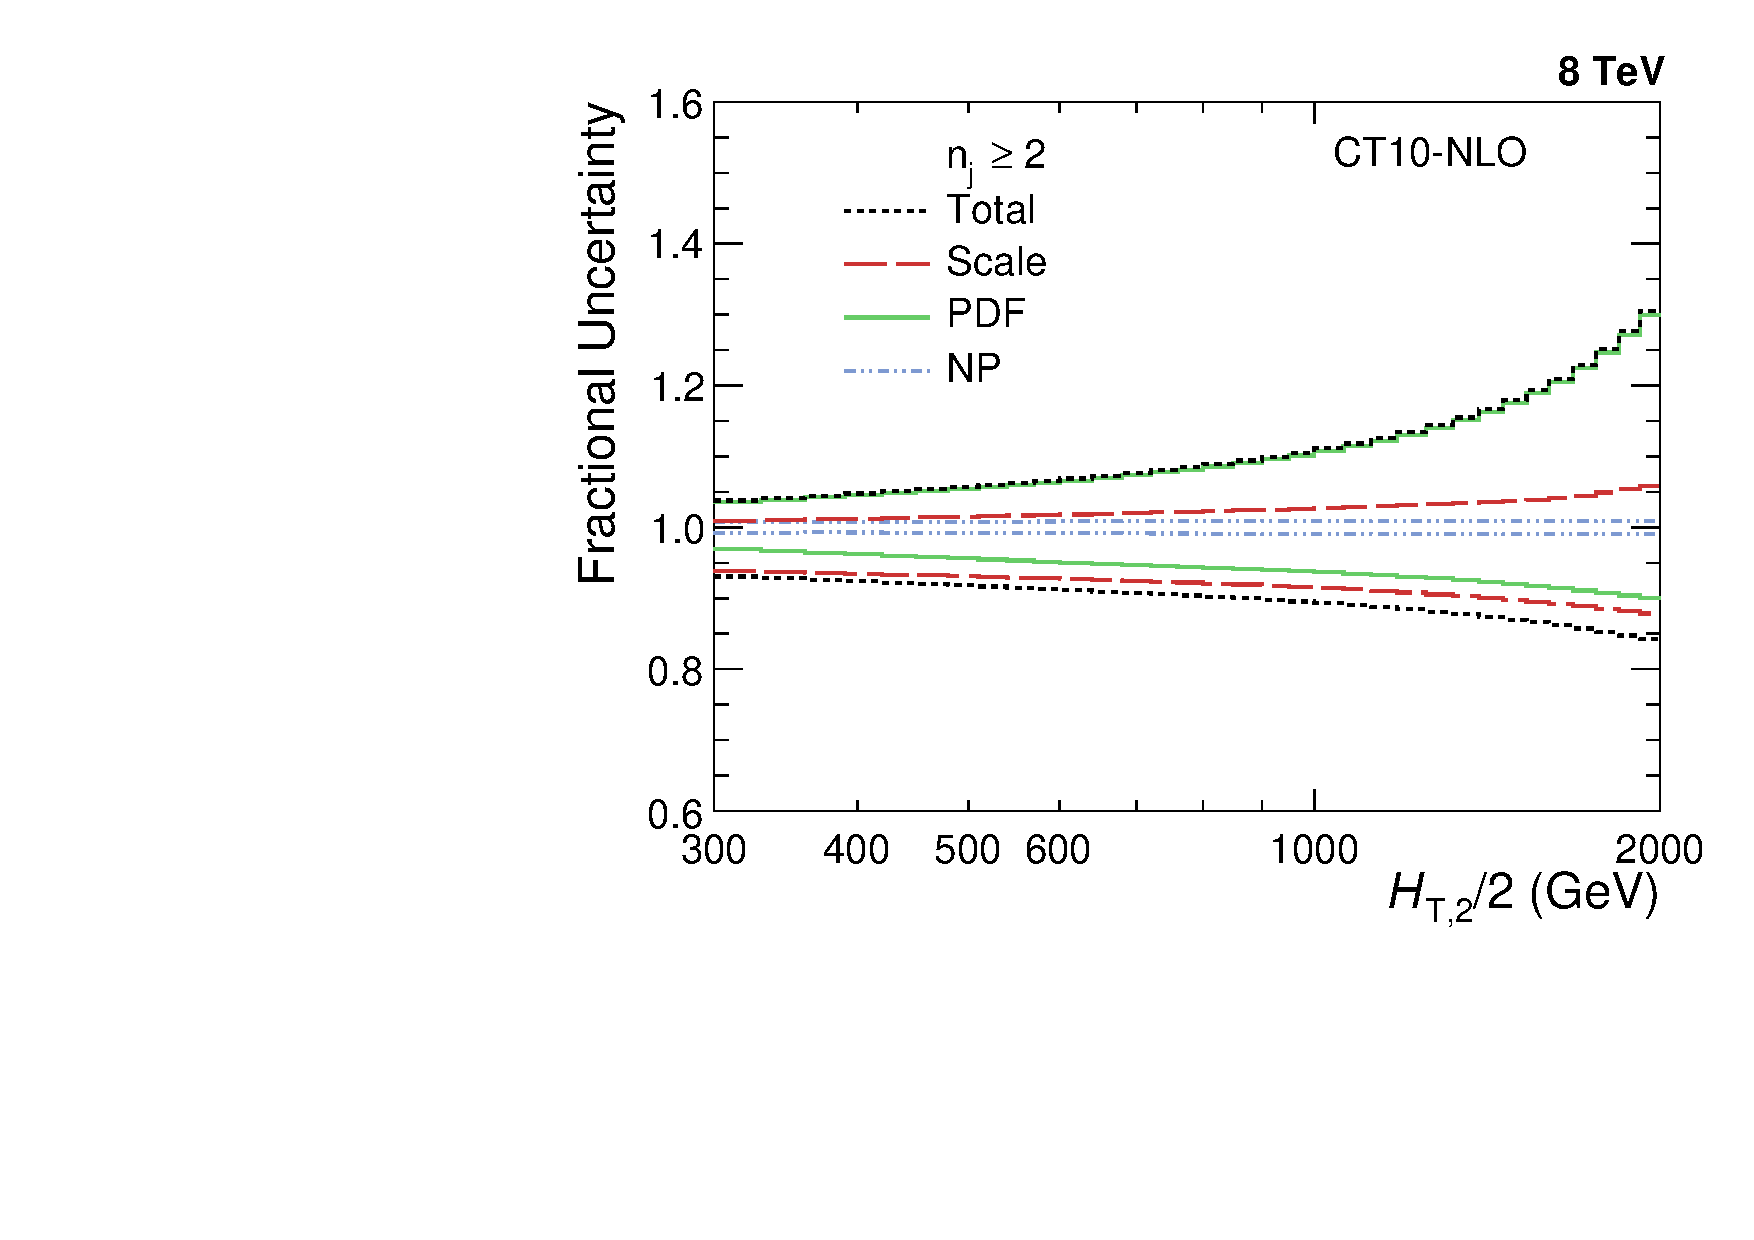
\includegraphics[width=0.51\textwidth]{Plots_HT_2_150/Theory_Unc_2.pdf}%
 ~~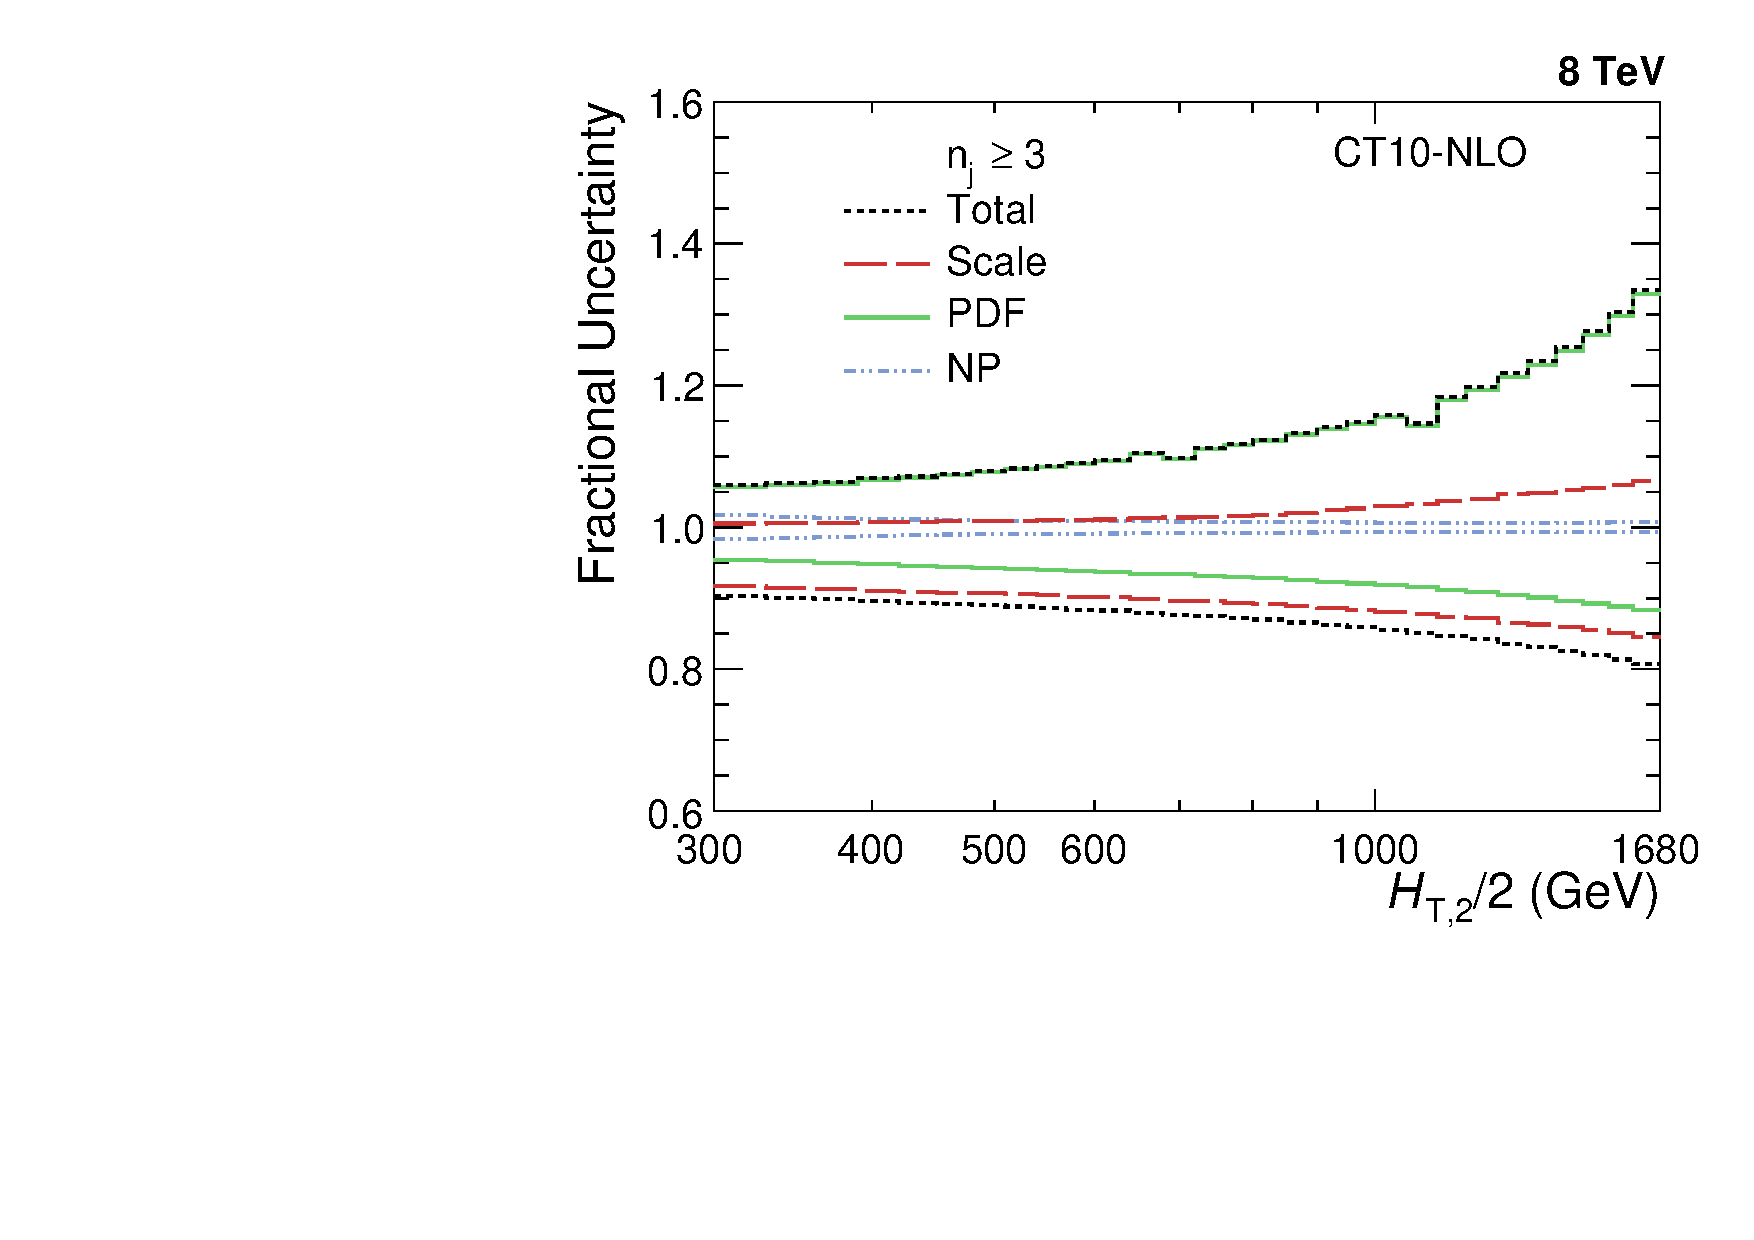
\includegraphics[width=0.51\textwidth]{Plots_HT_2_150/Theory_Unc_3.pdf}\\
 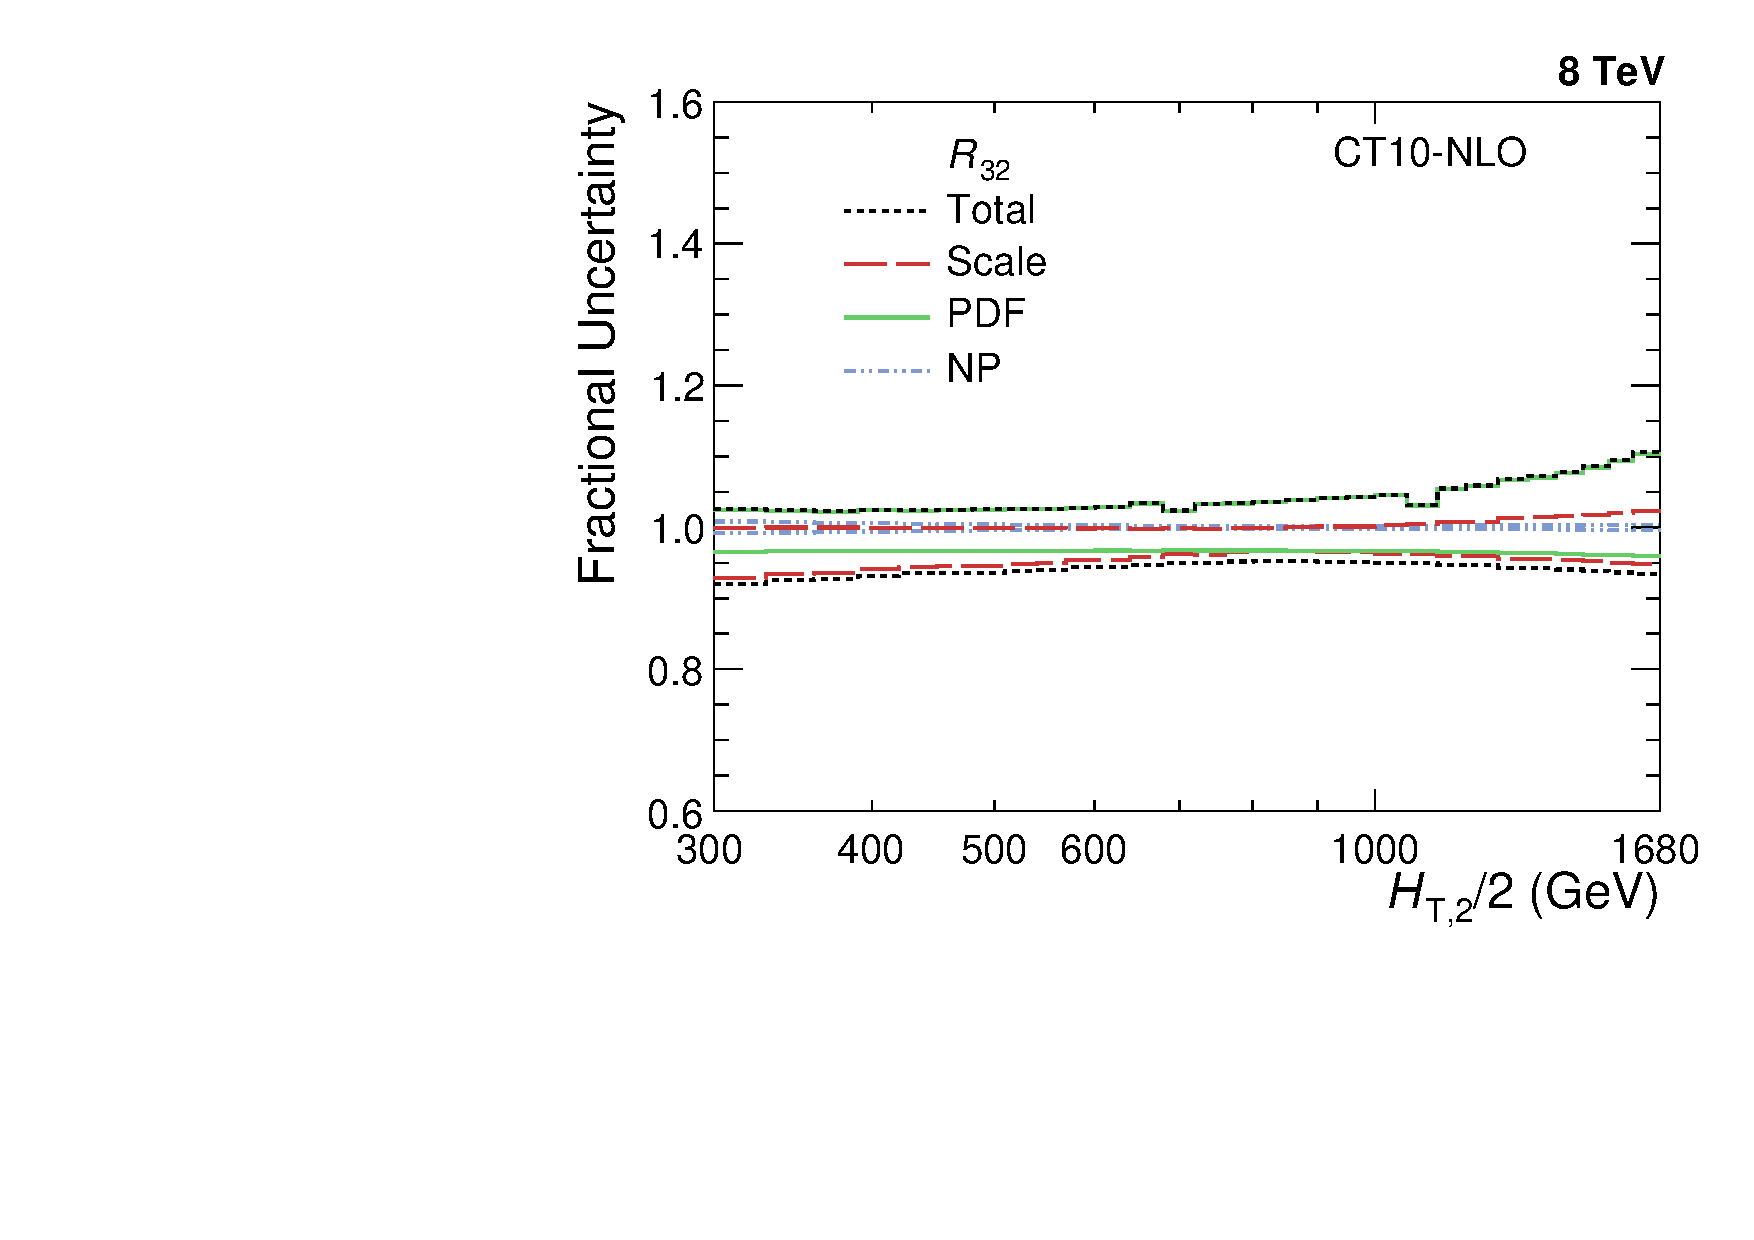
\includegraphics[width=0.51\textwidth]{Plots_HT_2_150/Theory_Unc_Ratio_32.pdf}\\
 \caption{The systematic theoretical uncertainties affecting the cross-section measurement for inclusive 2-jet (top left) and 3-jet events (top right) and their ratio \ratio (bottom). The scale (red dashed line), PDF (green line) and NP (blue dashed line) uncertainties as well as total uncertainty (black dashed line) obtained using CT10-NLO PDF set are shown. The total theoretical uncertainty is asymmetric and is dominated by PDF uncertainty.}
 \label{fig:theory_unc}
 \end{center}
\end{figure}

\subsection{Total Theoretical Uncertainty}
The total systematic theoretical uncertainties are obtained as the quadratic sum of the scale, PDF and NP uncertainties. Figure~\ref{fig:theory_unc} presents the systematic theoretical uncertainties affecting the cross-section measurement for inclusive 2-jet (top left) and 3-jet events (top right) and the cross-section ratio \ratio (bottom), using CT10-NLO PDF set. The scale (red dashed line), PDF (green line) and NP (blue dashed line) uncertainties as well as total theoretical uncertainty (black dashed line) are shown. The total theoretical uncertainty is asymmetric and is dominated by PDF uncertainty which grows in magnitude with increasing value of \httwo. Table~\ref{tab:theory_unc} quotes the values of the theoretical uncertainty from each source as well as total uncertainty affecting the measurements. The bin-wise values of uncertainties (in \%) from each source as well as total uncertainty are shown in Tables~\ref{tab:exp_unc2_th},~\ref{tab:exp_unc3_th} and~\ref{tab:exp_unc_ratio_th} for \njt~and \njth~event cross-sections and cross-section ratio \ratio, respectively. The computation of the NLO predictions with \NLOJETPP is also subject to statistical fluctuations from the complex numerical integrations. For the inclusive 2-jet event cross-sections this uncertainty is smaller than about a per mille, while for the inclusive 3-jet event cross-section it amounts to 1-9 per mille. Hence the statistical uncertainty is not considered in the total theoretical uncertainty. The small dips at $\sim$700 and 1000 GeV in the PDF uncertainty for inclusive 3-jet events cross-sections and cross-section ratio \ratio is a feature of the CT10-NLO PDF set.
 
\begin{table}[!h]
%\centering
 \caption{Overview of all systematic theoretical uncertainties, obtained using CT10-NLO PDF set, affecting the measurement of cross-sections for inclusive 2-jet (left) and 3-jet events (middle) and cross-section ratio \ratio (right).}
 \label{tab:theory_unc}
 \vspace{2mm}
 \begin{tabular}{lccc}
 \hline\hline
 {\bf Uncertainty Source}& {\bf Inclusive 2-jet} & {\bf Inclusive 3-jet} & {\bf \ratio} \rbthm\\ \hline
 Scale                   & 5 to 13\%             & 11 to 17\%            & 6 to 8\%  \rbtrr\\
 PDF                     & 3 to 30\%             & 4 to 32\%             & 2 to 10\% \rbtrr\\
 Non-perturbative (NP)   & 1\%                   & 1 to 2\%              & \ls 1\%   \rbtrr\\\hline
 Total                   & 3 to 30\%             & 5 to 34\%             & 3 to 11\% \rbtrr\\
 \hline\hline
 \end{tabular}
\end{table}

\section{Comparison of Theory to Data}
After correcting the measurement for detector effects as well as NLO pQCD calculations for non-perturbative (NP) and electroweak (EW) effects, it is now feasible to compare the measured cross-sections with the theory predictions. Figure~\ref{fig:data_NL0_MC} shows the measured differential inclusive 2-jet and 3-jet event cross-sections as a function of \httwo after unfolding for detector effects. On the left, the measurements (points) are compared to the \NLOJETPP predictions using the CT10-NLO PDF set (line), corrected for NP effects and in addition for EW effects in the 2-jet case. On the right, the comparison is made to the predictions from \MadGraphFn \plusn \PYTHIAS (MG\plusn P6) with tune \Ztwostar (line), corrected for EW effects in the 2-jet case. The error bars give the total experimental uncertainty, given by the quadrature sum of the statistical and systematic uncertainties. On a logarithmic scale, the data are in well agreement with the NLO predictions over the whole range of \httwo from 300 GeV up to 2000 (2-jet) and 1680 GeV (3-jet) respectively. 

\begin{figure}[!h]
 \hspace*{-5mm}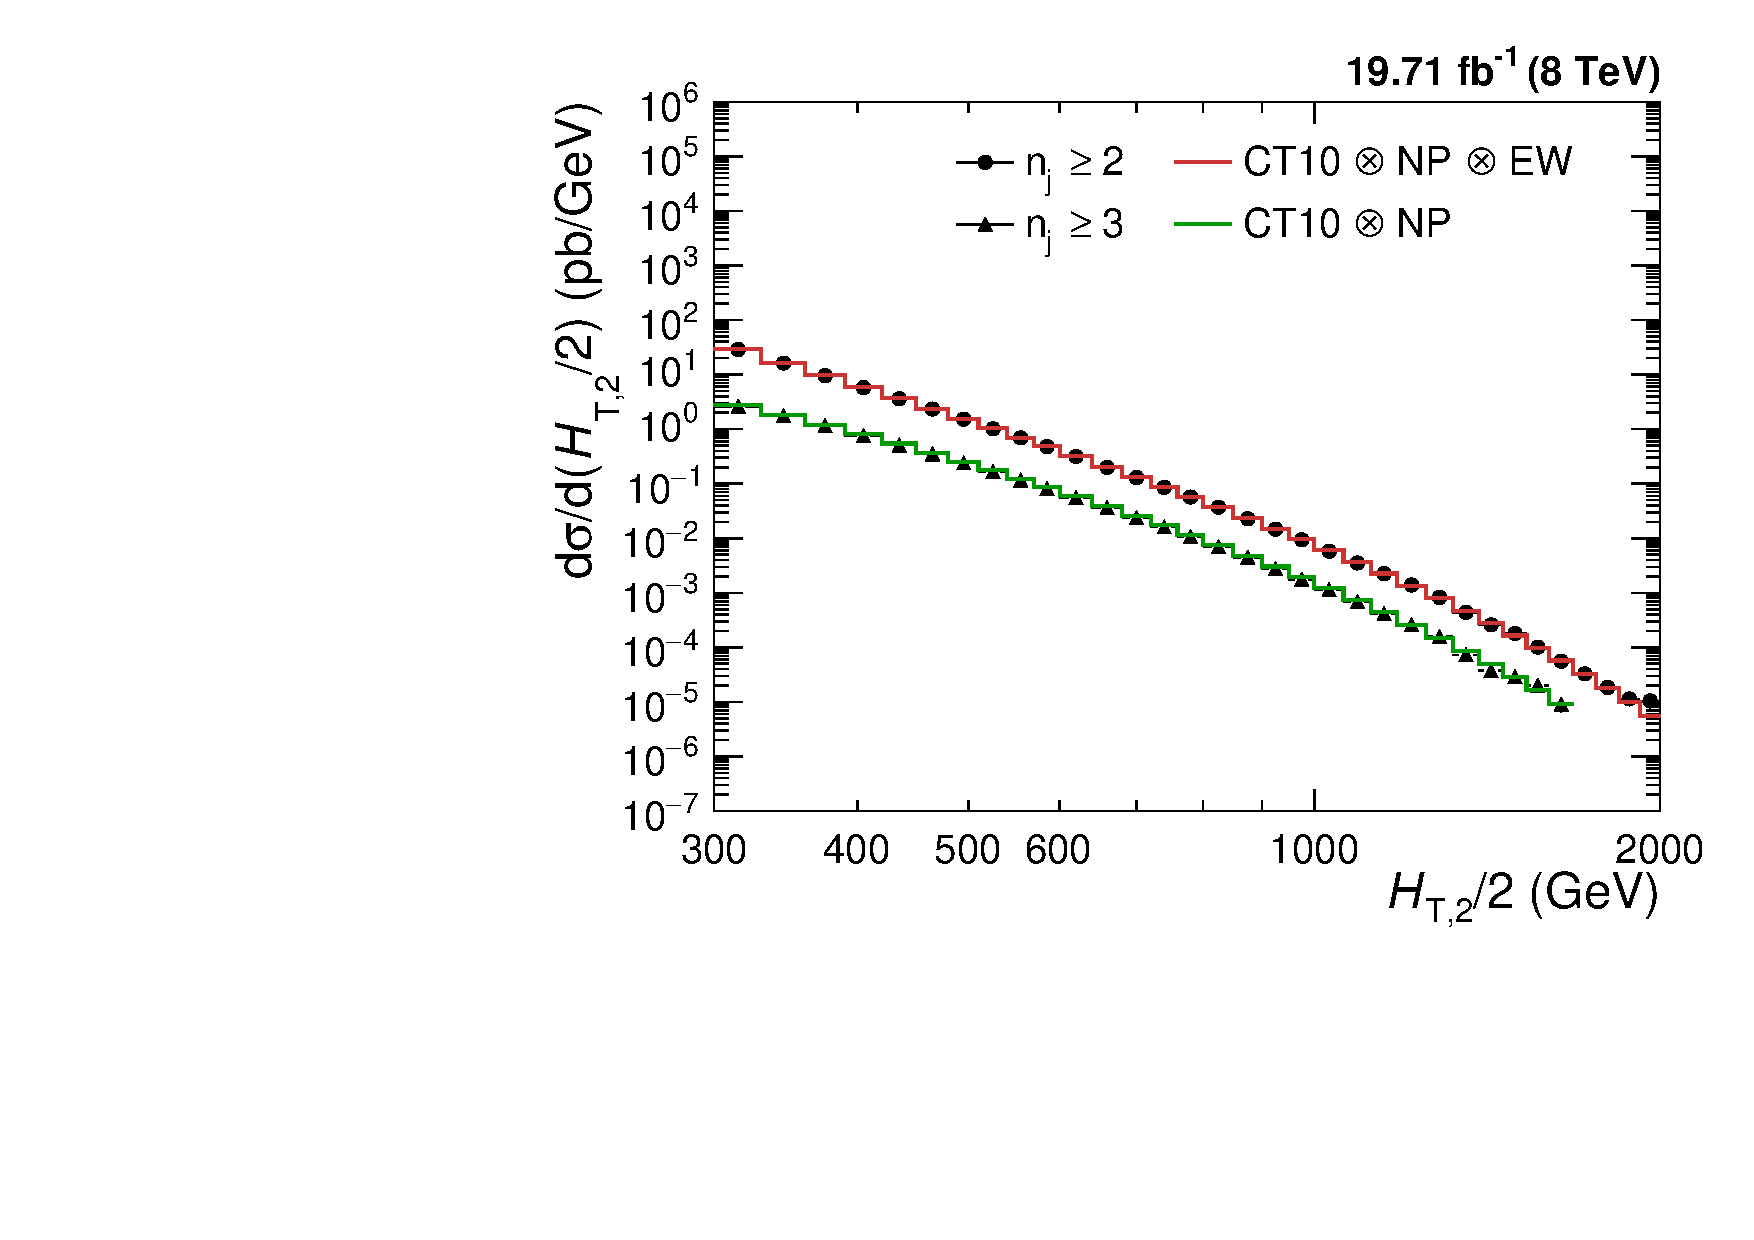
\includegraphics[width=0.51\textwidth]{Plots_HT_2_150/Comparison_data_theory_EW.pdf}%
 ~~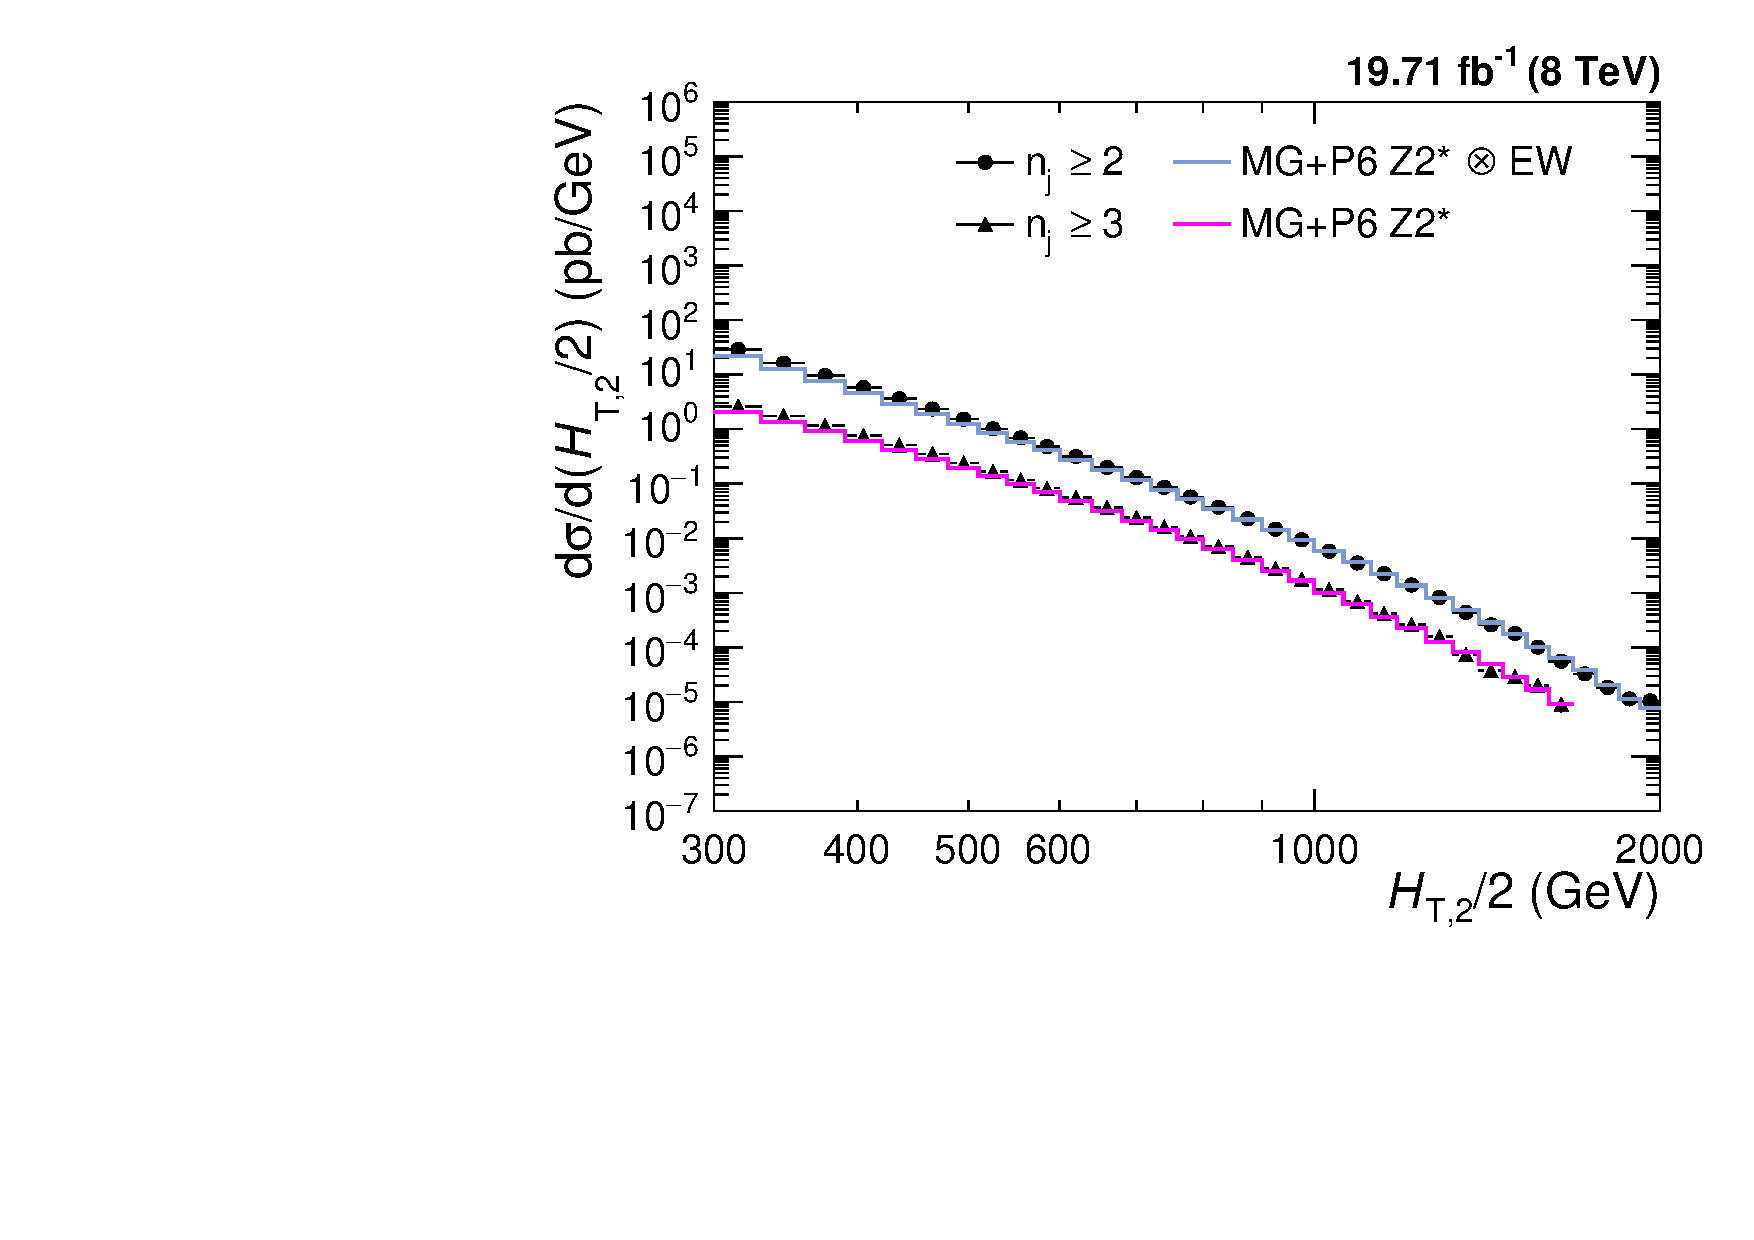
\includegraphics[width=0.51\textwidth]{Plots_HT_2_150/Comparison_data_MC_EW.pdf}\\
 \caption[]{Comparison of the measured differential inclusive 2-jet and 3-jet event cross-sections as a function of \httwo to theoretical predictions. On the left, the data (points) are shown together with \NLOJETPP predictions (line) using the CT10-NLO PDF set, corrected for non-perturbative (NP) and electroweak (EW) effects (2-jet) or only NP effects (3-jet). On the (right), the data (points) are compared to predictions from \MadGraphFn \plusn \PYTHIAS (MG\plusn P6) with tune \Ztwostar (line), corrected for EW effects in the 2-jet case. The error bars give the total experimental uncertainty, given by the quadrature sum of the statistical and systematic uncertainties.}
 \label{fig:data_NL0_MC}
\end{figure}

\begin{figure}[!h]
 \begin{center}
 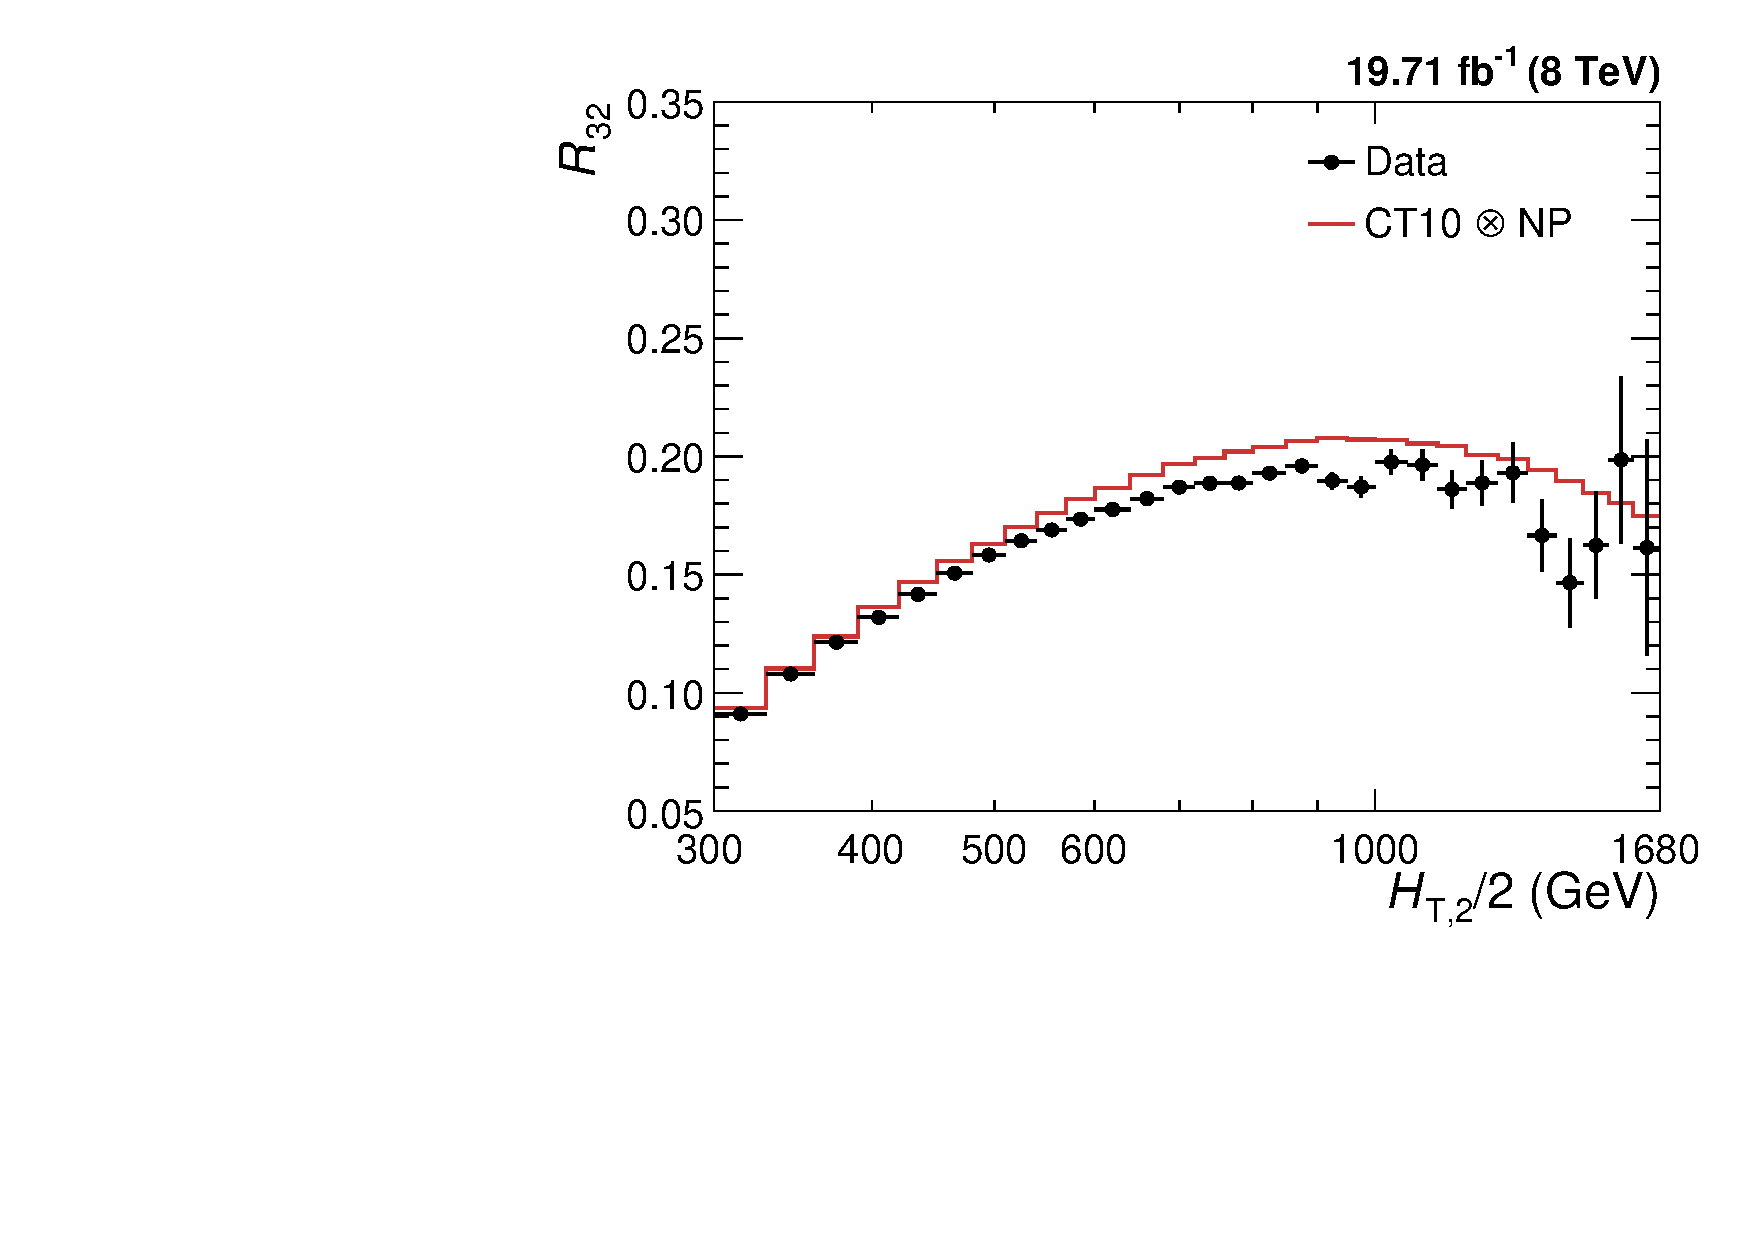
\includegraphics[width=0.50\textwidth]{Plots_HT_2_150/Sensitivity_ratio_32_CT10_only.pdf}%
 \caption{Cross-section ratio \ratio as a function of \httwo calculated from data (solid circles) in comparison to that from NLO pQCD predictions obtained using the CT10-NLO PDF set corrected with non-perturbative (NP) corrections (line). The error bars correspond to the total experimental uncertainty derived as quadratic sum from all uncertainty sources.}
 \label{fig:ratiosens}
 \end{center}
\end{figure}

Figure~\ref{fig:ratiosens} shows the cross-section ratio \ratio obtained from unfolded data data (solid circles) in comparison to that from NLO pQCD predictions obtained using the CT10-NLO PDF set corrected with NP corrections (line). The error bars here represents the total experimental uncertainty derived as quadratic sum from all uncertainty sources. The deviations of measured \ratio from the theoretical predicted value can be explained by the electroweak effects which are not considered yet because of their unavailability for inclusive 3-jet event cross-sections.

\begin{figure}[!ht]
 \begin{center}
 \hspace*{-5mm}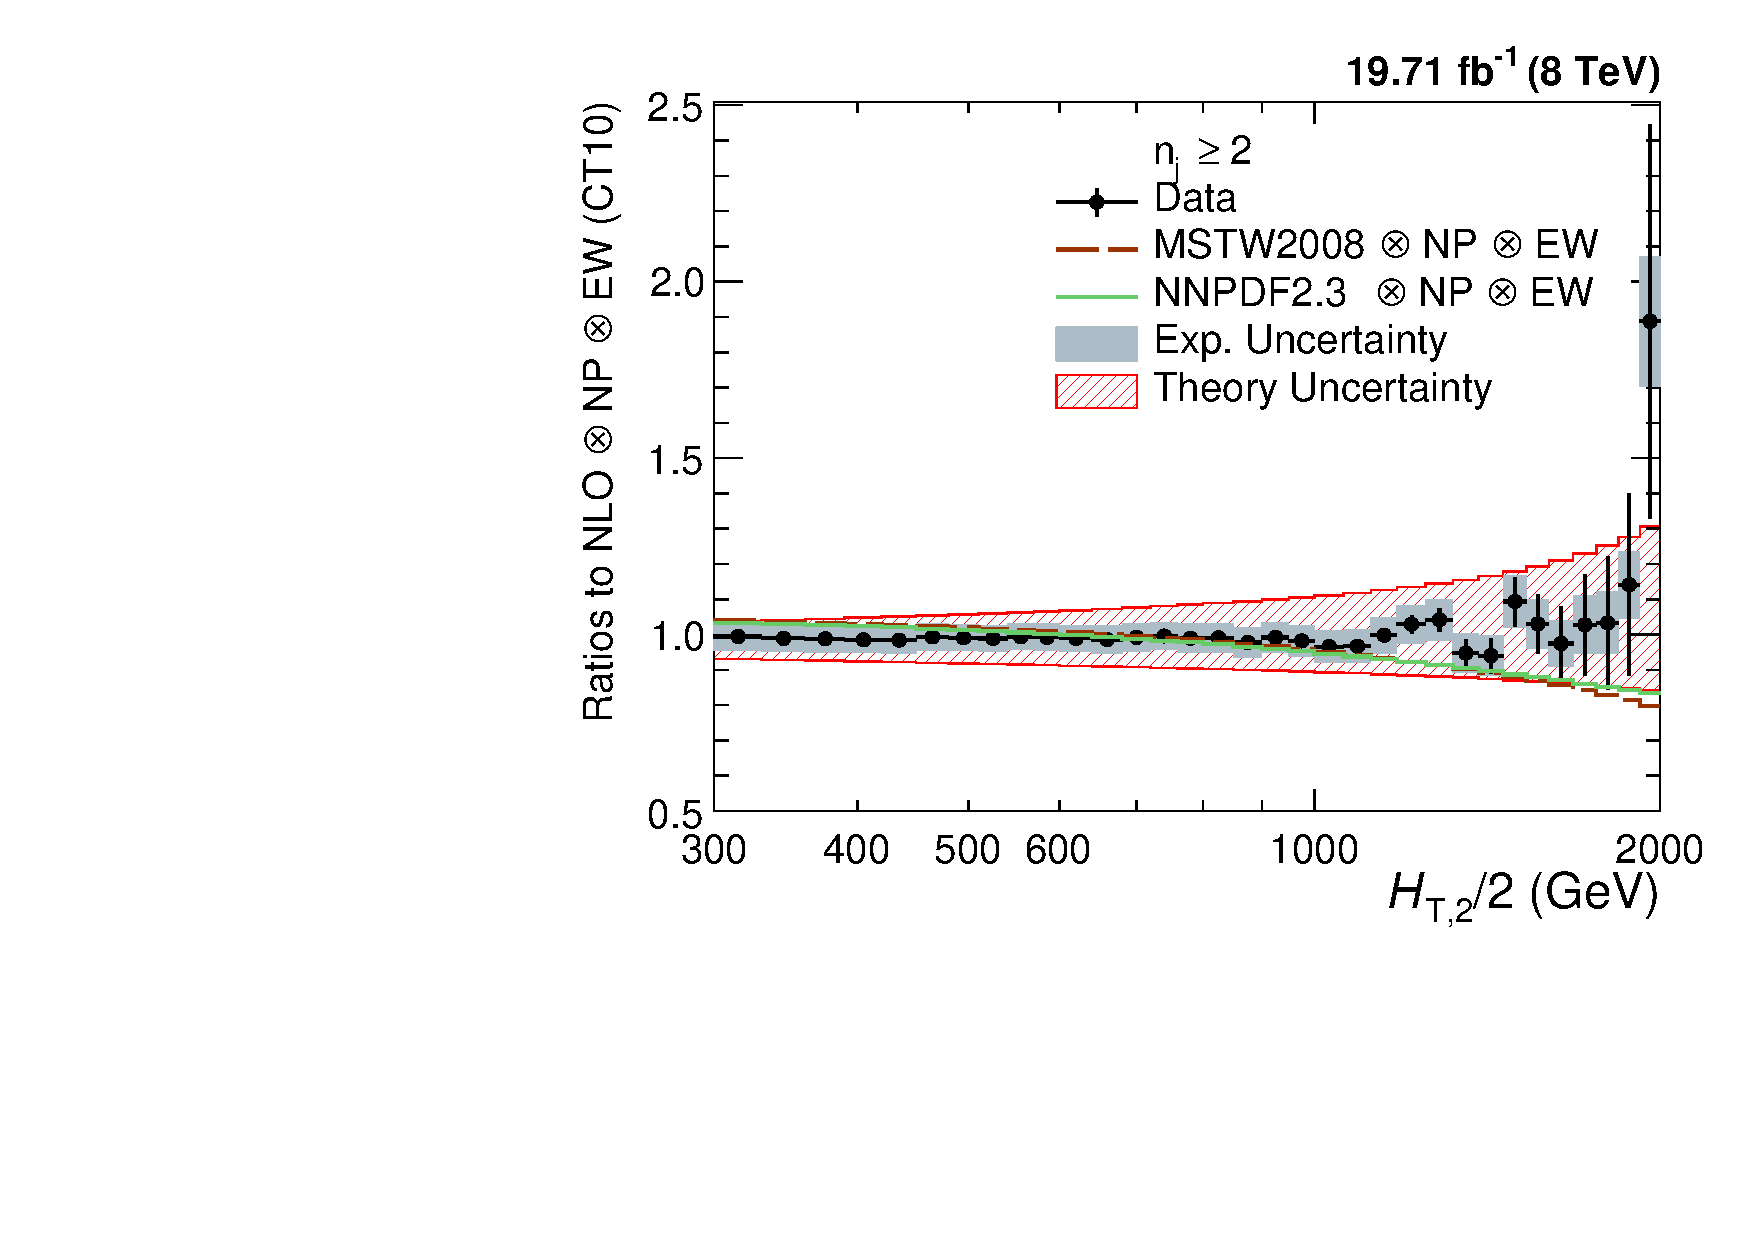
\includegraphics[width=0.51\textwidth]{Plots_HT_2_150/Comparison_data_NLO_Pdfs_2_EW.pdf}%
 ~~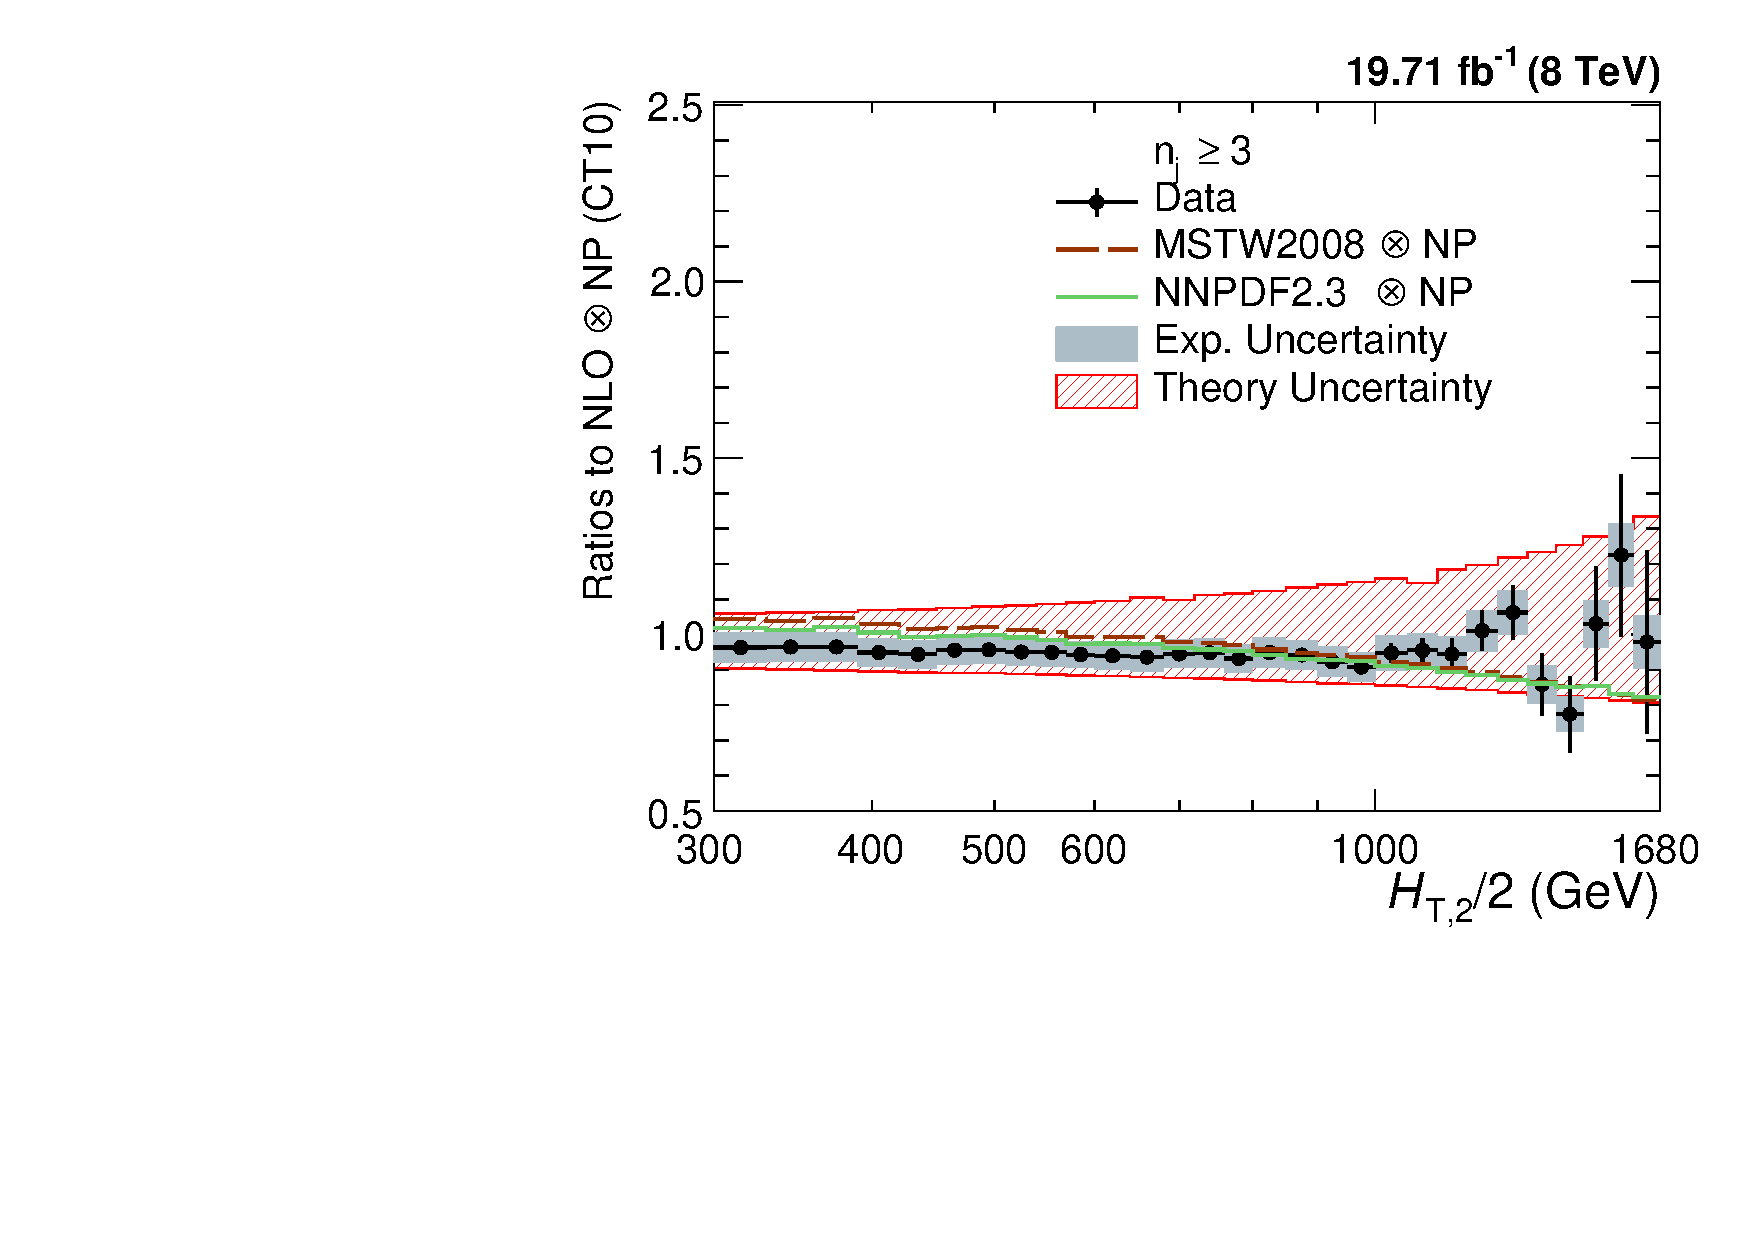
\includegraphics[width=0.51\textwidth]{Plots_HT_2_150/Comparison_data_NLO_Pdfs_3.pdf}\\
 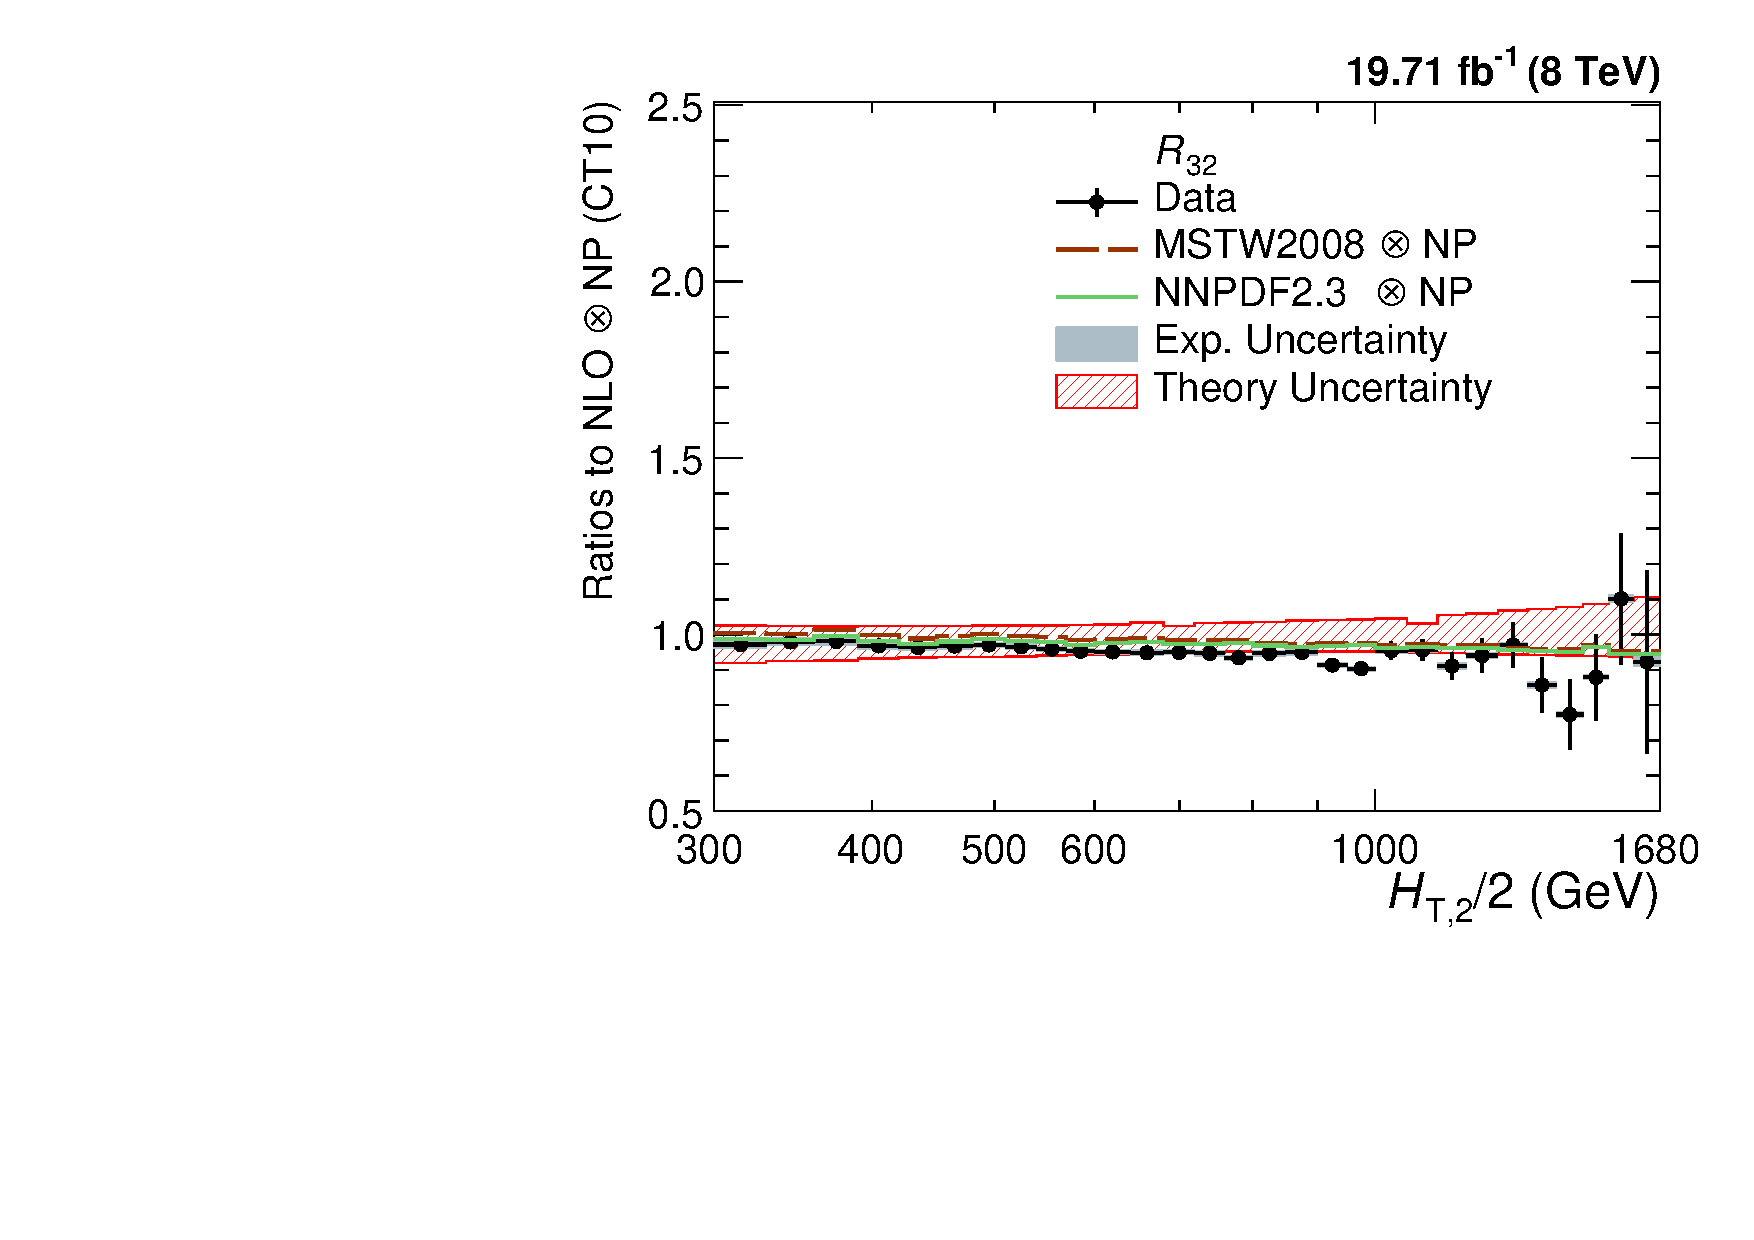
\includegraphics[width=0.51\textwidth]{Plots_HT_2_150/Comparison_data_NLO_Pdfs_ratio_32.pdf}\\
 \caption{Ratio of data over theory using the CT10-NLO PDF set for inclusive 2-jet (top left) and 3-jet event cross-sections (top right) and their ratio \ratio (bottom). The theory predictions are corrected for non-perturbative effects (NP) and also for electroweak effects (EW) for inclusive 2-jet only. For comparison predictions employing two other PDF sets, MSTW2008 and NNPDF2.3, are also shown. The error bars represents the statistical uncertainty of the data and the shaded rectangles represents the total experimental systematic uncertainty. The shaded band around unity indicate the total uncertainty of the theory.}
 \label{fig:data_NLOPdfs}
 \end{center}
\end{figure}

For better visibility, the ratios of data over the theory at NLO are also studied in details. In Fig.~\ref{fig:data_NLOPdfs}, the ratios of data over \NLOJETPP predictions using the CT10-NLO PDF set are shown for inclusive 2-jet (top left) and 3-jet event cross-sections (top right) as well as their ratio \ratio (bottom). The data are well described by the predictions within their uncertainty, which is dominated at large \httwo by PDF effects in the upwards and by scale variations in the downwards direction. A trend towards an increasing systematic excess of the 2-jet data with respect to theory, starting at about 1\TeV in \httwo, is remedied by the inclusion of EWK corrections. In the 3-jet case the statistical precision of the data and the reach in \httwo is insufficient to observe any effect. The alternative PDF sets MSTW2008 and NNPDF2.3 exhibit a small underestimation of the cross-sections at high \httwo.

\begin{figure}[!h]
 \begin{center}
 \hspace*{-5mm}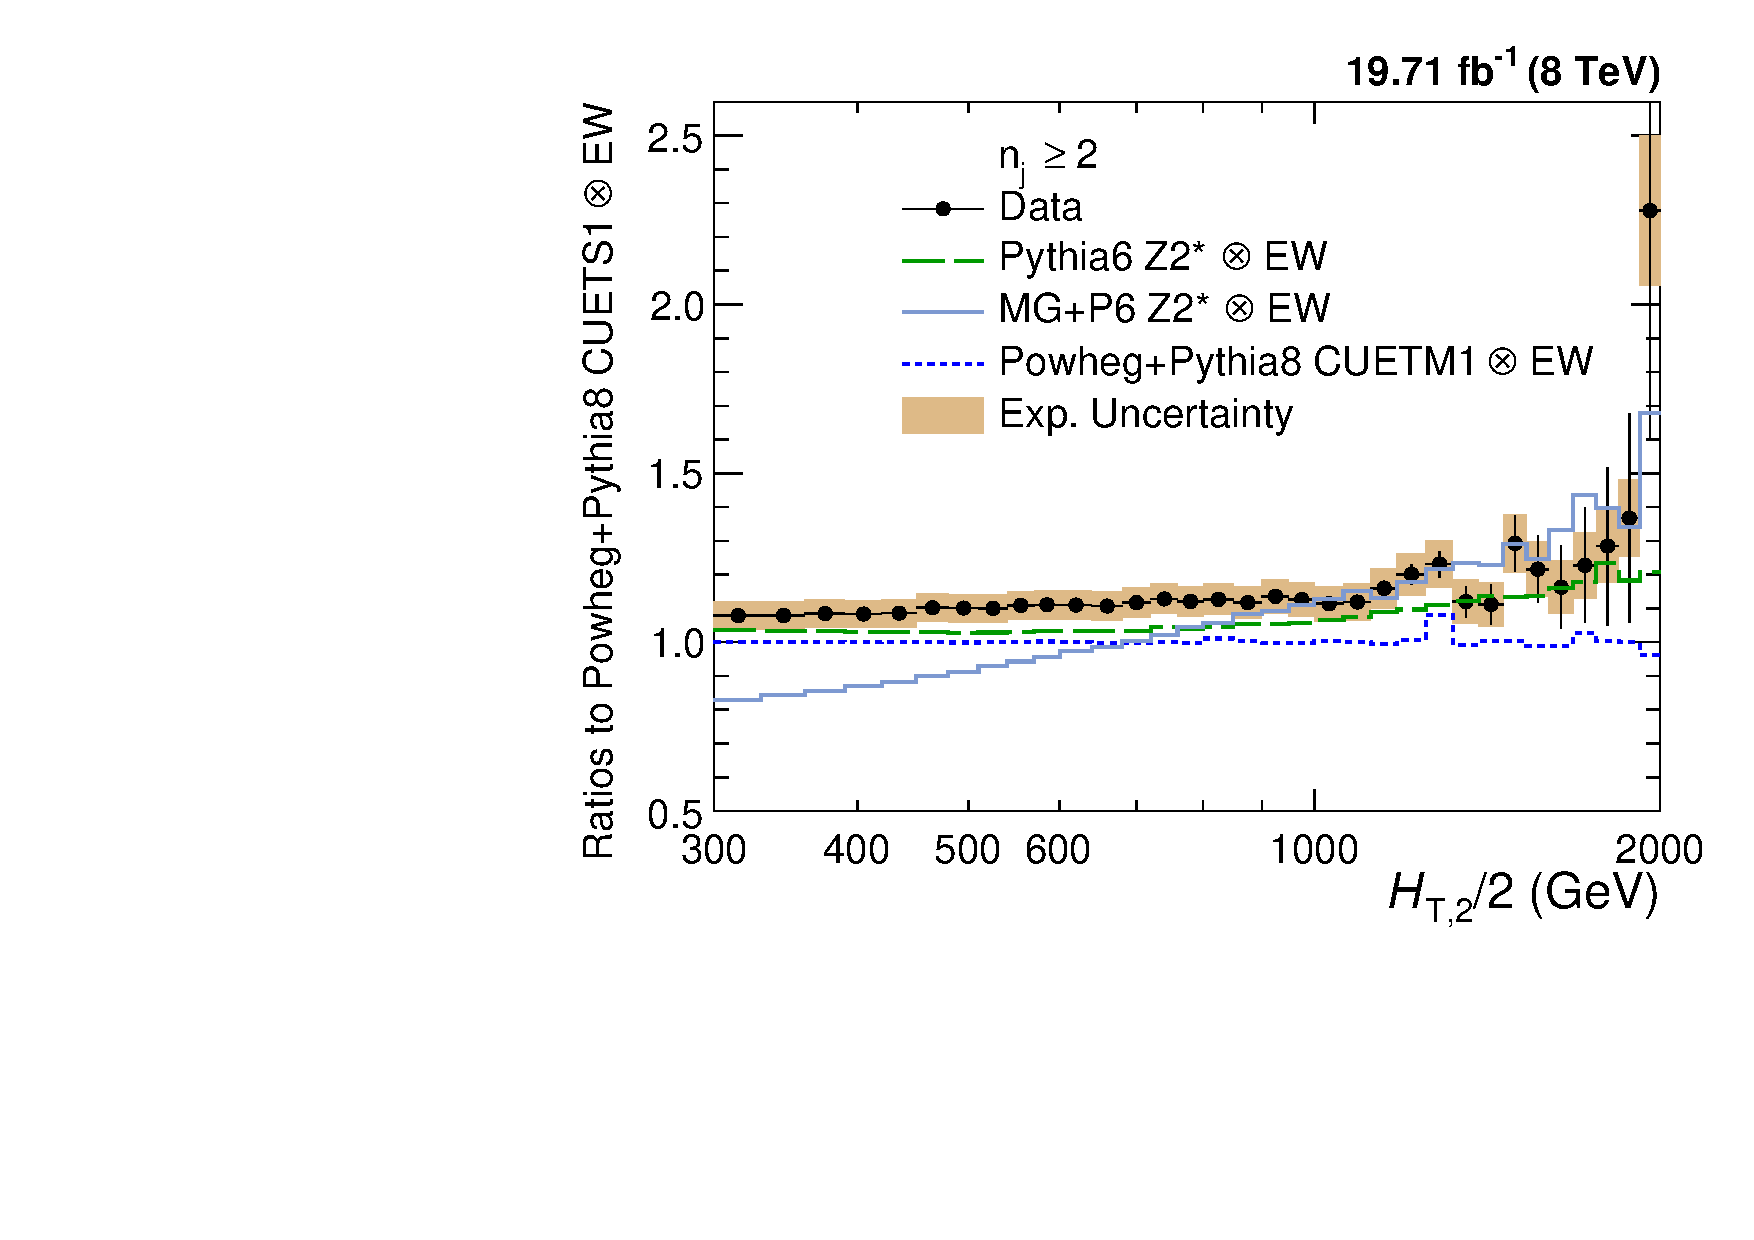
\includegraphics[width=0.51\textwidth]{Plots_HT_2_150/Comparison_data_MC_samples_2_Pow_EW.pdf}%
 ~~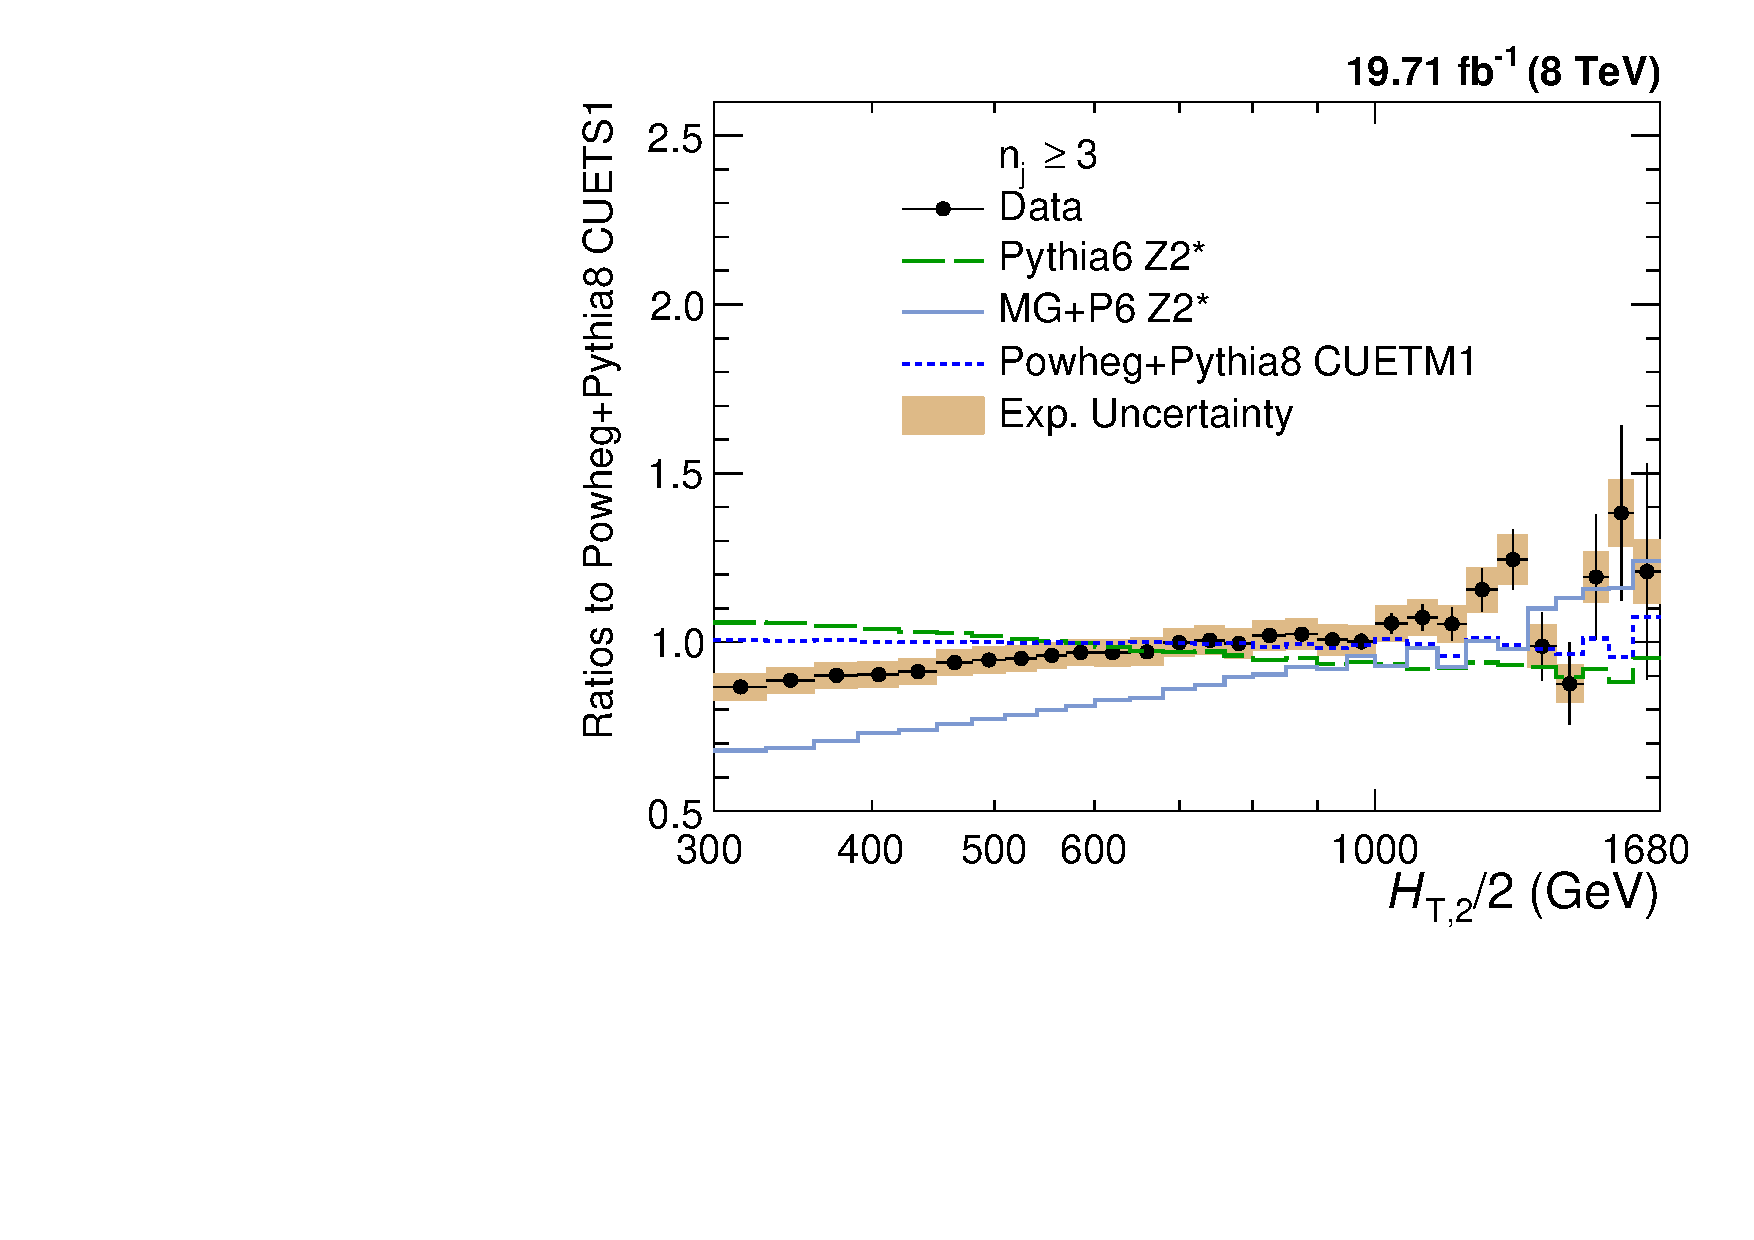
\includegraphics[width=0.51\textwidth]{Plots_HT_2_150/Comparison_data_MC_samples_3_Pow.pdf}\\
 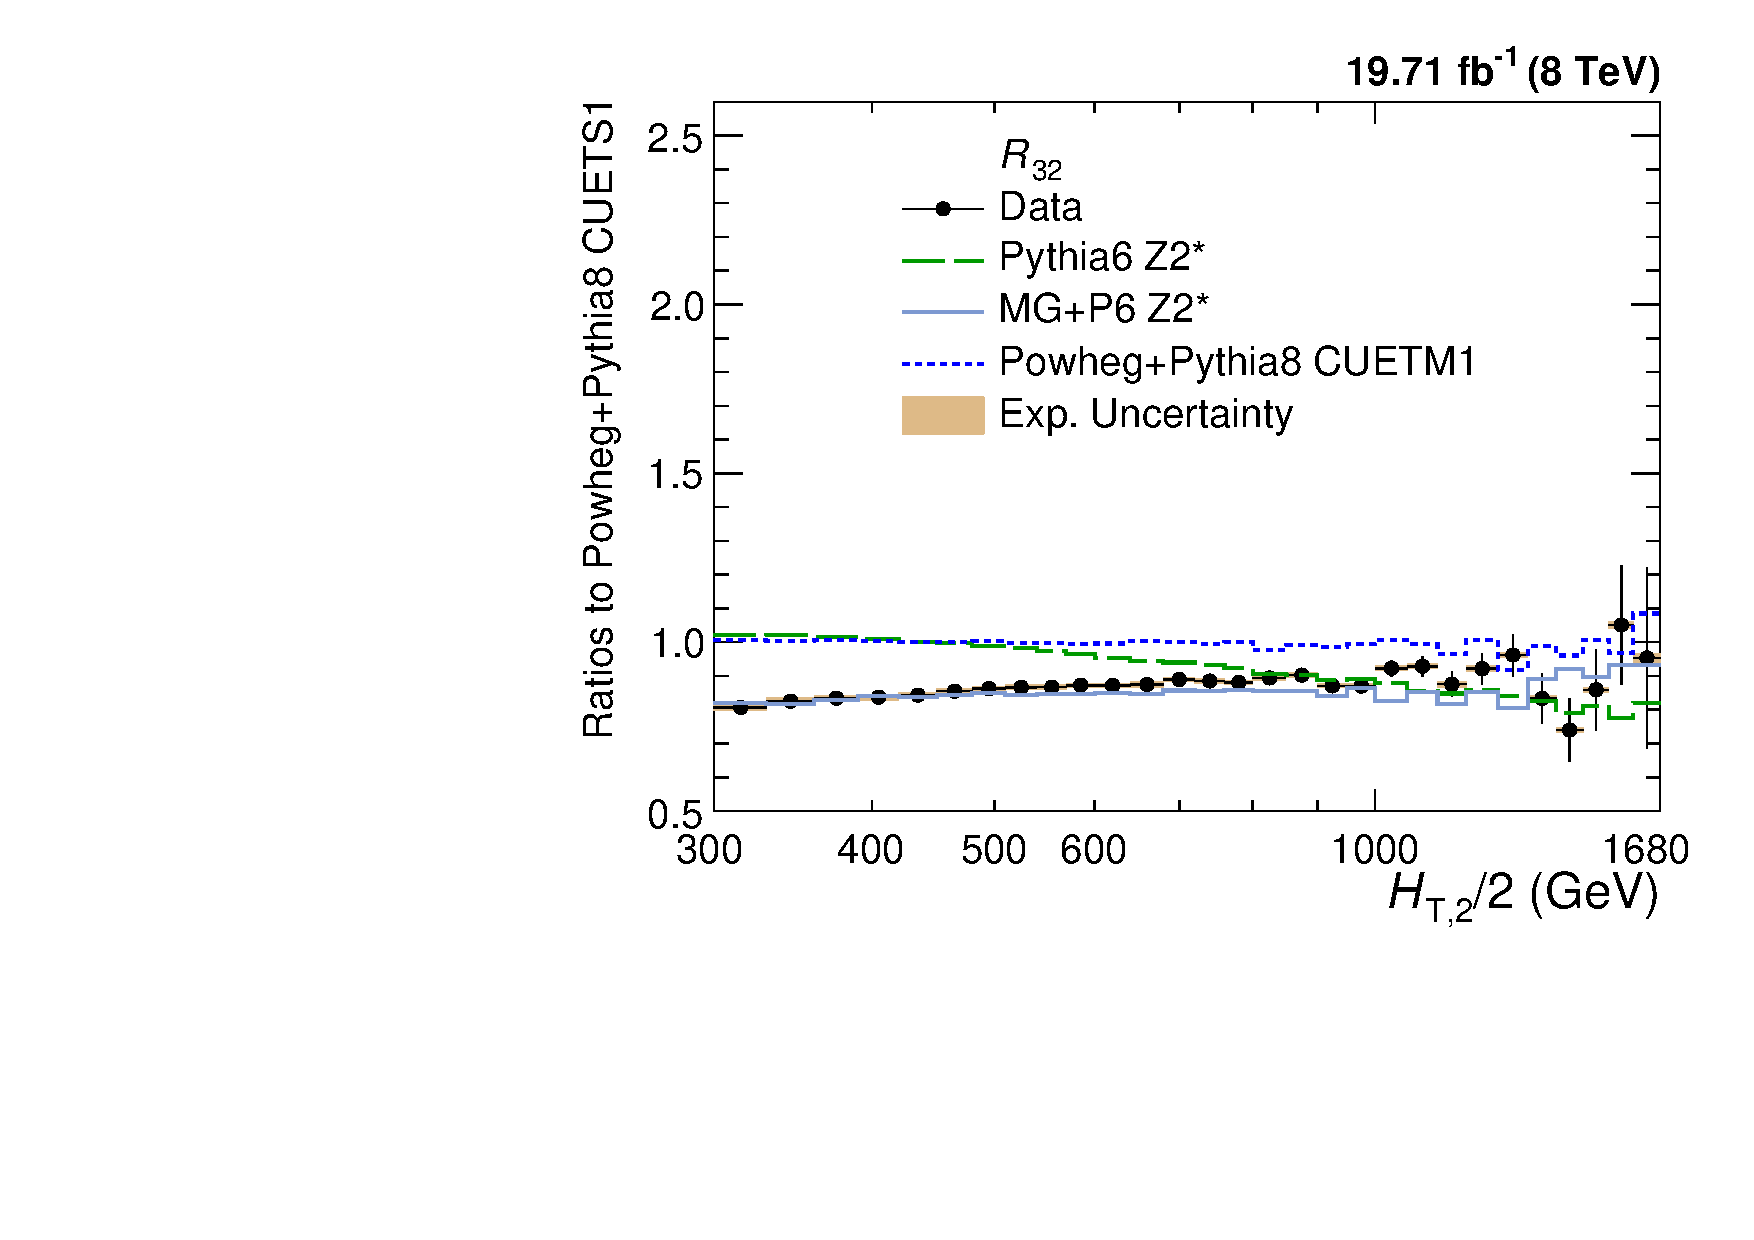
\includegraphics[width=0.51\textwidth]{Plots_HT_2_150/Comparison_data_MC_samples_ratio_32_Pow.pdf}\\
 \caption[]{Ratio of data over the prediction from \POWHEGn \plusn \PYTHIAE with tune CUETS1 are presented for inclusive 2-jet (top left) and 3-jet event cross-sections (top right) as well as their ratio \ratio (bottom). For comparison the alternative tune CUETM1 of \POWHEGn \plusn \PYTHIAE, the tree-level multi-leg improved prediction by \MadGraphFn \plusn \PYTHIAS with tune \Ztwostar, and the the LO MC predictions from \PYTHIAS tune \Ztwostar are shown as well. The error bars correspond to the statistical uncertainty of the data and the shaded rectangles to the total experimental systematic uncertainty. EW corrections have been accounted for in this comparison in the 2-jet case only.}
 \label{fig:data_MC}
 \end{center}
\end{figure}

The \POWHEG~framework providing a NLO dijet calculation matched to the parton showers of \PYTHIAE employed with the CUETS1 and CUETM1 tunes \cite{Khachatryan:2015pea} is also used for a comparison. The ratios of data over theory from \POWHEGn \plusn \PYTHIAE with tune CUETS1 are shown for inclusive 2-jet (top left) and 3-jet event cross-sections (top right) as well as their ratio \ratio (bottom) in Fig.~\ref{fig:data_MC}. For comparison, the LO prediction from \PYTHIAS with tune \Ztwostar, the tree-level multi-leg improved prediction by \MadGraphFn \plusn \PYTHIAS with tune \Ztwostar, and the matched NLO prediction from \POWHEGn \plusn \PYTHIAE with tune CUETM1 are shown as well. EW corrections have been accounted for in this comparison in the 2-jet case only. Significant discrepancies, which are cancelled to a large extent in the ratio \ratio, are visible in the comparison with the LO prediction from \MadGraphFn \plusn \PYTHIAS with tune \Ztwostar, in particular for small \httwo. In contrast, the employed dijet MC \POWHEGn \plusn \PYTHIAE better describe the 2-jet event cross-section, but fail for the 3-jet case.

The jet measurements at hadron colliders can be used to extract the strong coupling constant \alps, which is discussed in the next chapter.

